\chapter{Boats and Sailing}


\section{Boats}
Engineers have been building boats for centuries.  Through boat design, humanity learned the lessons that made airplanes and rockets possible.
Learning about how boats work will give you a foundation for understanding more advanced concepts we will be covering later.

\subsection{Basic Terminology}
\index{bough}
\index{hull}
The front of a boat is called \newterm{the bow} (pronounced exactly the same as "bough"). The back of the boat is called \newterm{the stern}.

The underside of the boat is called \newterm{the hull}.  The top of the boat is called \newterm{the deck}.

\begin{center}
    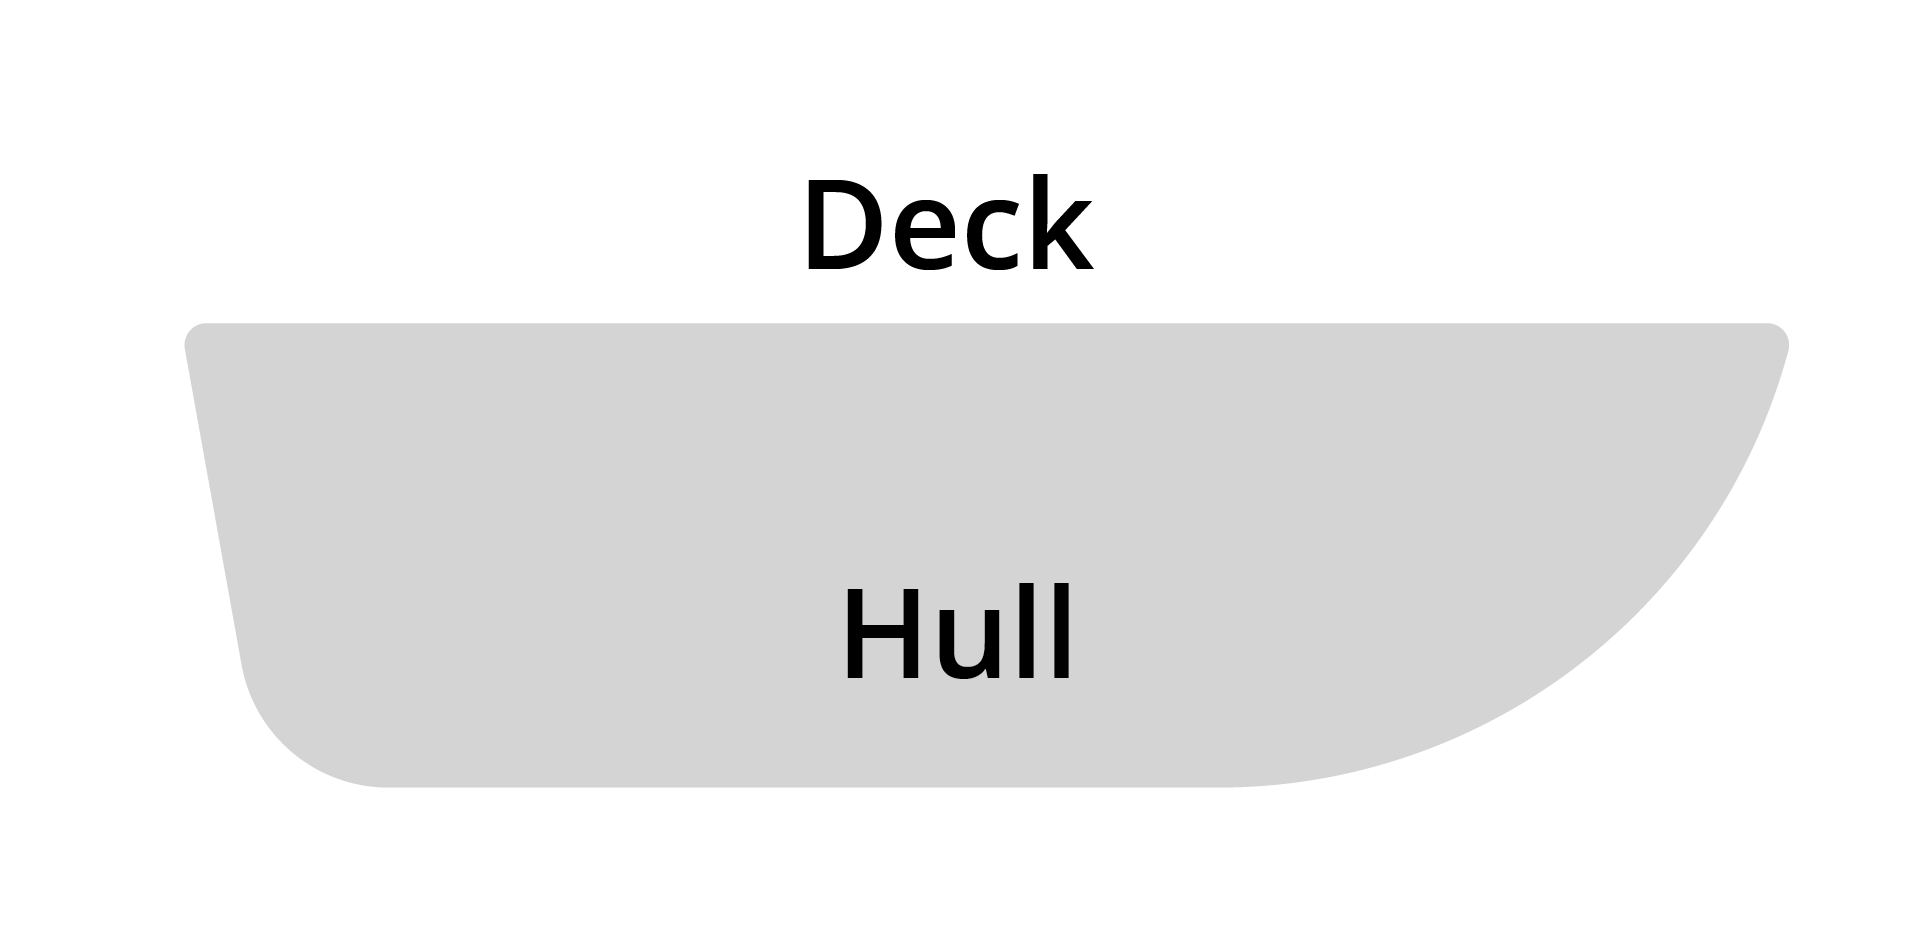
\includegraphics[width=.75\textwidth]{deckHull.png}

\end{center}
\index{stern}
\index{port}
\index{starboard}

If you are standing at the stern and looking toward the bow, everything on your left is the \newterm{port} side.  Everything on your right is the \newterm{starboard} side.

\begin{center}
    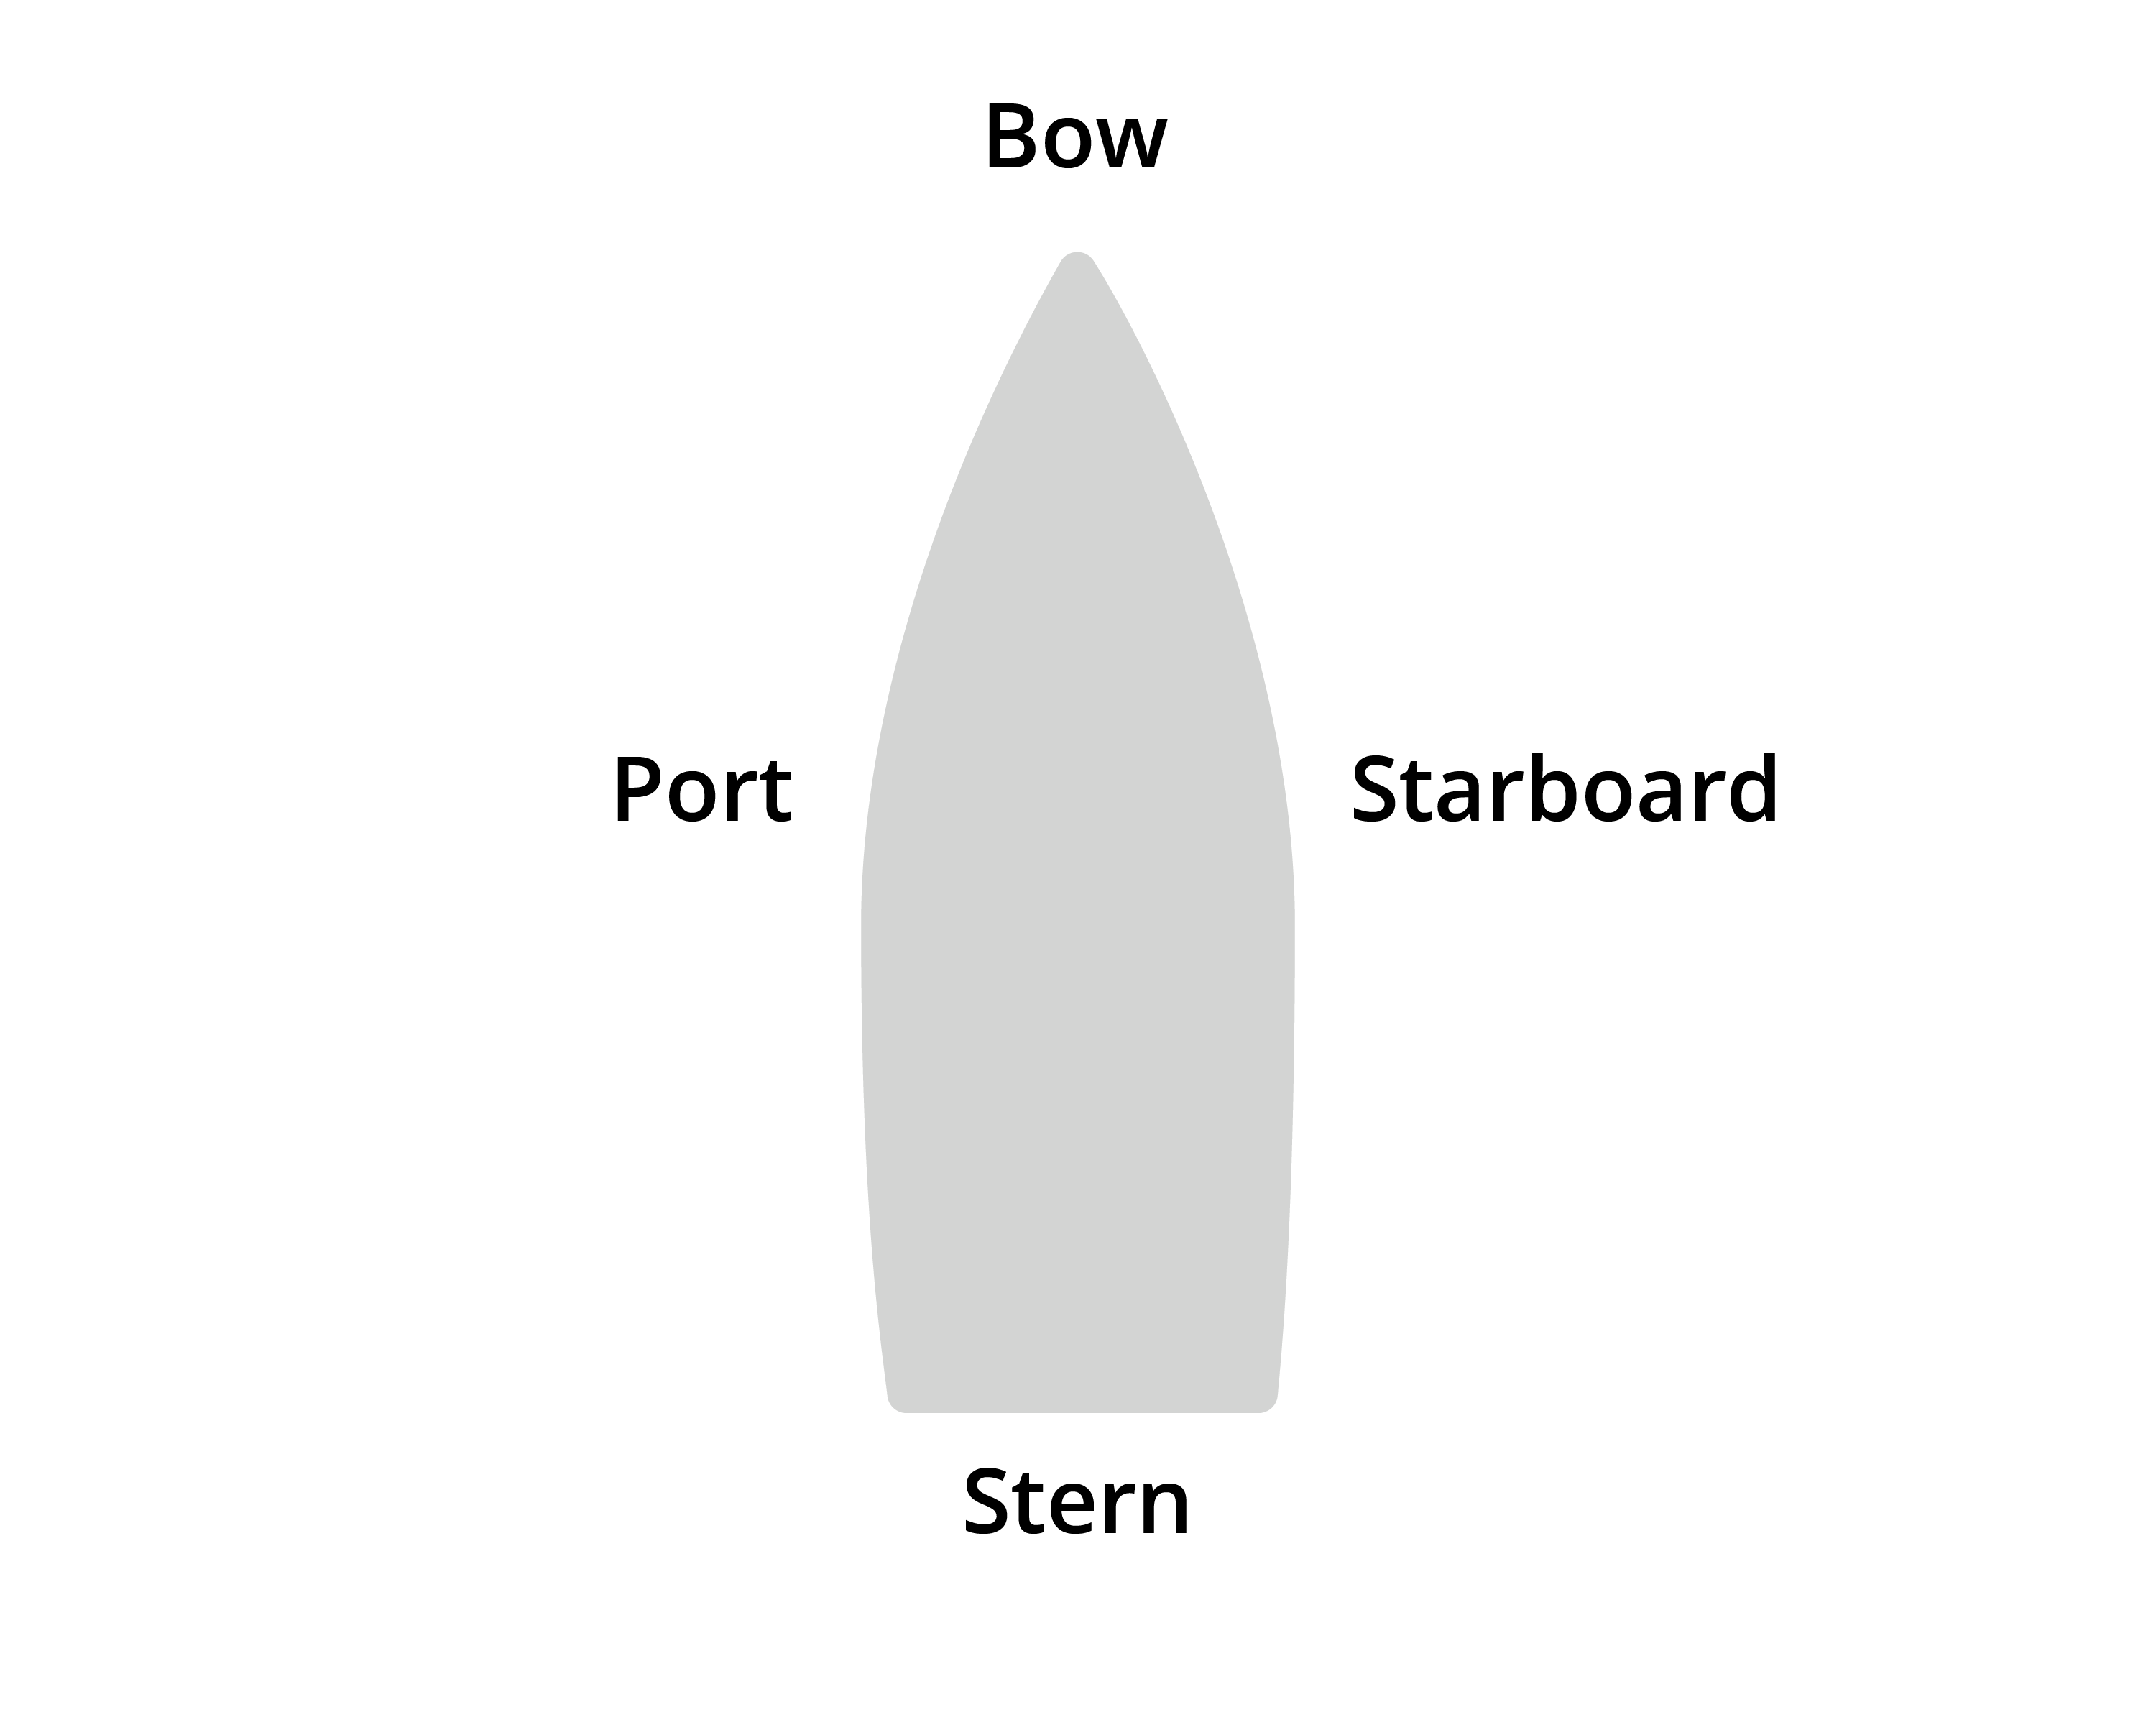
\includegraphics[width=.75\textwidth]{bowStern.png}

\end{center}
There are several different ways that boats are propelled:

\begin{itemize}


\item A motor turns a screw in the water, as in a motorboat. The screw is known as a \newterm{propeller}. \index{propeller}

\item A human pushes the water with a big spatula.  If the spatula is attached to the boat with a pivot (as in a rowboat) it is an \newterm{oar}.  If the spatula is not attached to the boat (as in a canoe), it is a \newterm{paddle}.

\item A human pushes the ground beneath the water with a long pole. These boats are called \newterm{punts}, and are mainly used in more shallow waters where an oar or a paddle would be less convenient.

\item The wind pushes the boat,  as in a sailboat. The sails are held up by a \newterm{mast}.
\index{sail}
\index{mast}
\item Some boats have a big fan that propel the boat.  These are called \newterm{airboats}\index{airboats}.   Airboats are not the most efficient boats,  but they can travel
on waterways with water just a couple of inches deep.

\begin{center}
    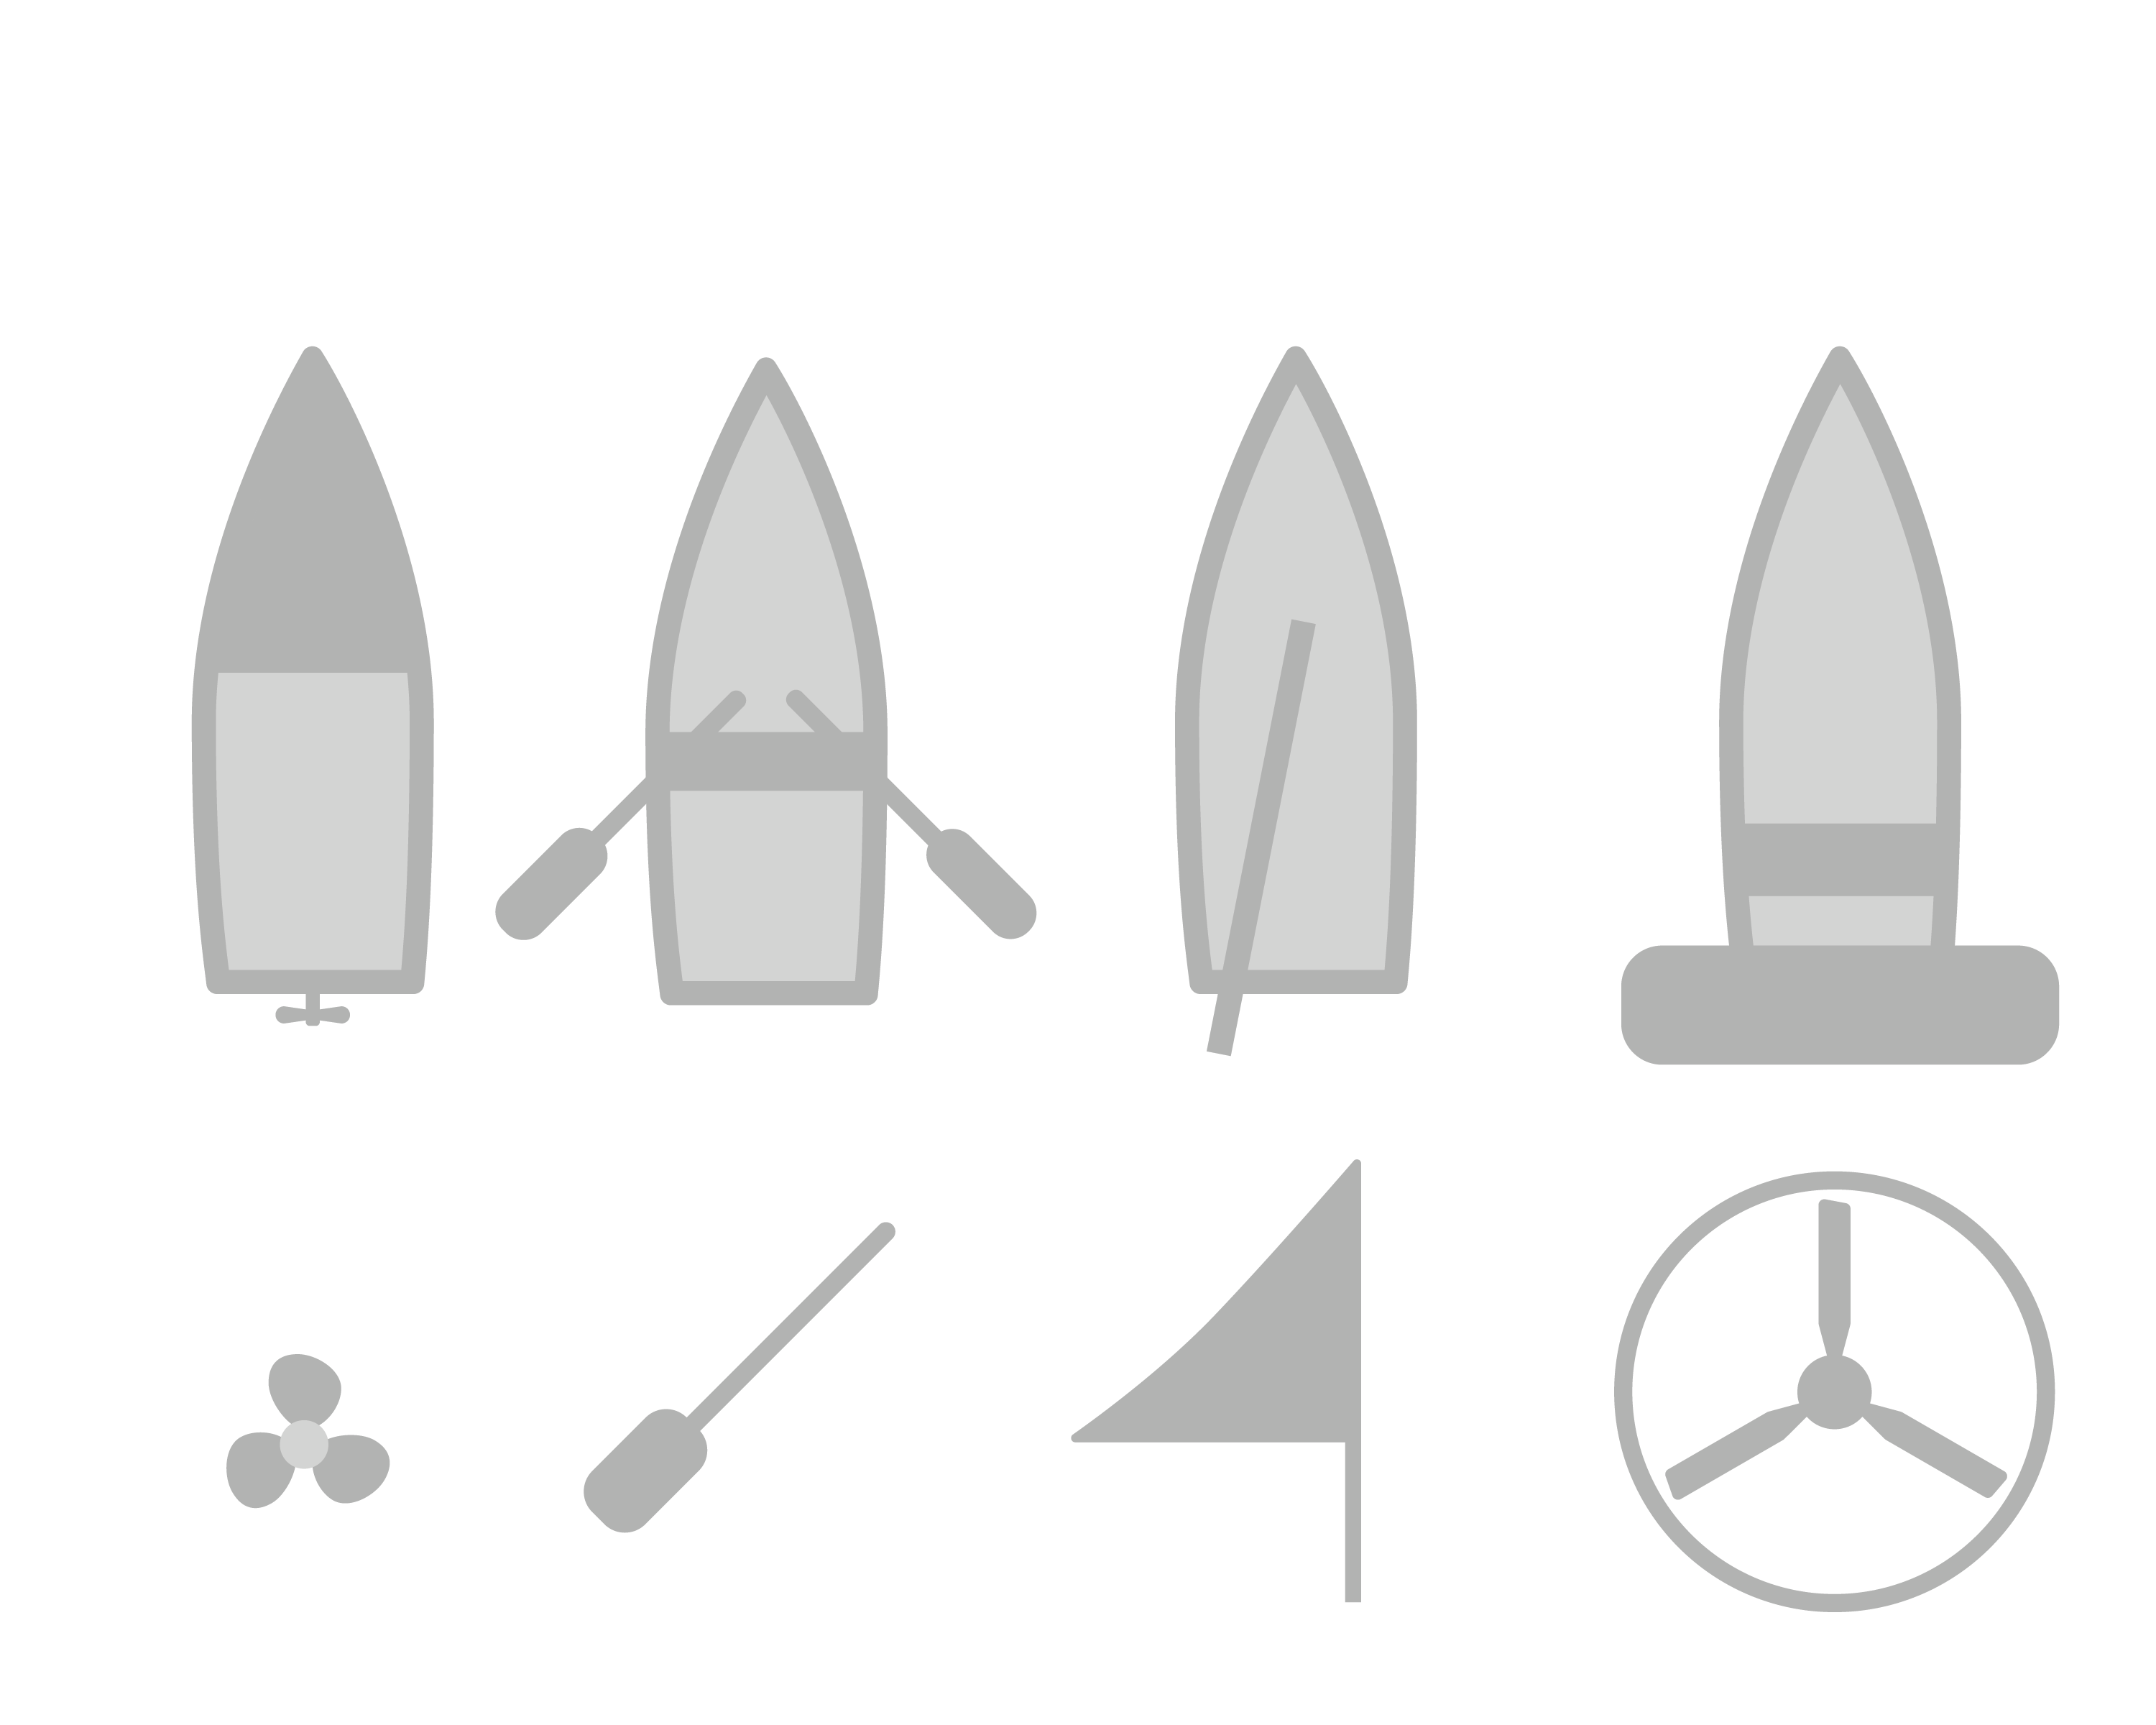
\includegraphics[width=.75\textwidth]{boatTypes.png}

\end{center}

\end{itemize}

In the terms of physics, each of these method provide a \newterm{thrust vector}\index{thrust vector} which is applied to the boat at a particular place and in a particular direction.

\subsubsection{Nautical Miles and Knots}

A \newterm{nautical mile}\index{nautical mile} is use to measure distances on a boat. The speed of a boat is usually measured in \newterm{knots}\index{knots}, which is just a quick way of saying "nautical miles per hour".

What is a nautical mile?

Latitude is the angle that a boat is above or below the equator. It is measured in degrees, minutes, and seconds. 60 minutes make one degree. 60 seconds make one minute.  So, for example, if you are $12.45164^\circ$ north of the equator, a sailor might say you were at Latitude $12^\circ 27' 5" N$.  She might also say that you are a little more than 747 nautical miles from the equator. ($12 \times 60 + 27 = 747$)

A nautical mile is the distance of one minute of latitude. It is slightly longer than the normal (or \newterm{statute}) that you use on land: one nautical mile equals 1.151 statute miles or 1.852 km per hour.

\subsection{Why Boats Float Upright}

Early in this sequence, we discussed buoyancy as a quantity. The magnitude of the buoyant force is equivalent to the weight of the liquid displaced.

We can also talk about the direction of the buoyant force: buoyancy pushes in the opposite direction as gravity.

How do we design boats so that they don't flip over?

\subsubsection{Center of Buoyancy}

Let's say you have a rowboat. If you push down on point on the floor near the front, the front of the boat will go down and the back of the boat will rise. In other words, the boat will rotate in the direction you are pushing.
Likewise, if you push on the floor near the back of the boat, the back will sink a little lower and the front will rise. However, there is a place, near the center of the boat, where if you push down, the boat will not rotate at all; it will simply sink a little lower
in the water. That point is known as the \newterm{center of buoyancy}.
\index{center of buoyancy}

How can we calculate the center of buoyancy?  Imagine the shape of the water that was displaced by the boat. Now imagine that shape filled with water. The center of mass of that water is the center of buoyancy of the boat.

\subsubsection{Center of Mass}
\index{center of mass}
Your boat and everything in it can be thought of as one object.  That object has a center of mass. If you found the center of mass, you could balance the whole boat on it.

In a boat,  if you move your body from the center of the boat to once side, you will have moved the center of mass. The boat will lean in that direction, which will change the center of buoyancy.

If you imagine a line is parallel to the force of gravity that passes through the center of mass of your boat, the boat will continue to increase its lean until
the center of buoyancy is on that line.

If water comes over the sides of the boat before the center of gravity and center of buoyancy align, your boat will sink.

\begin{center}
    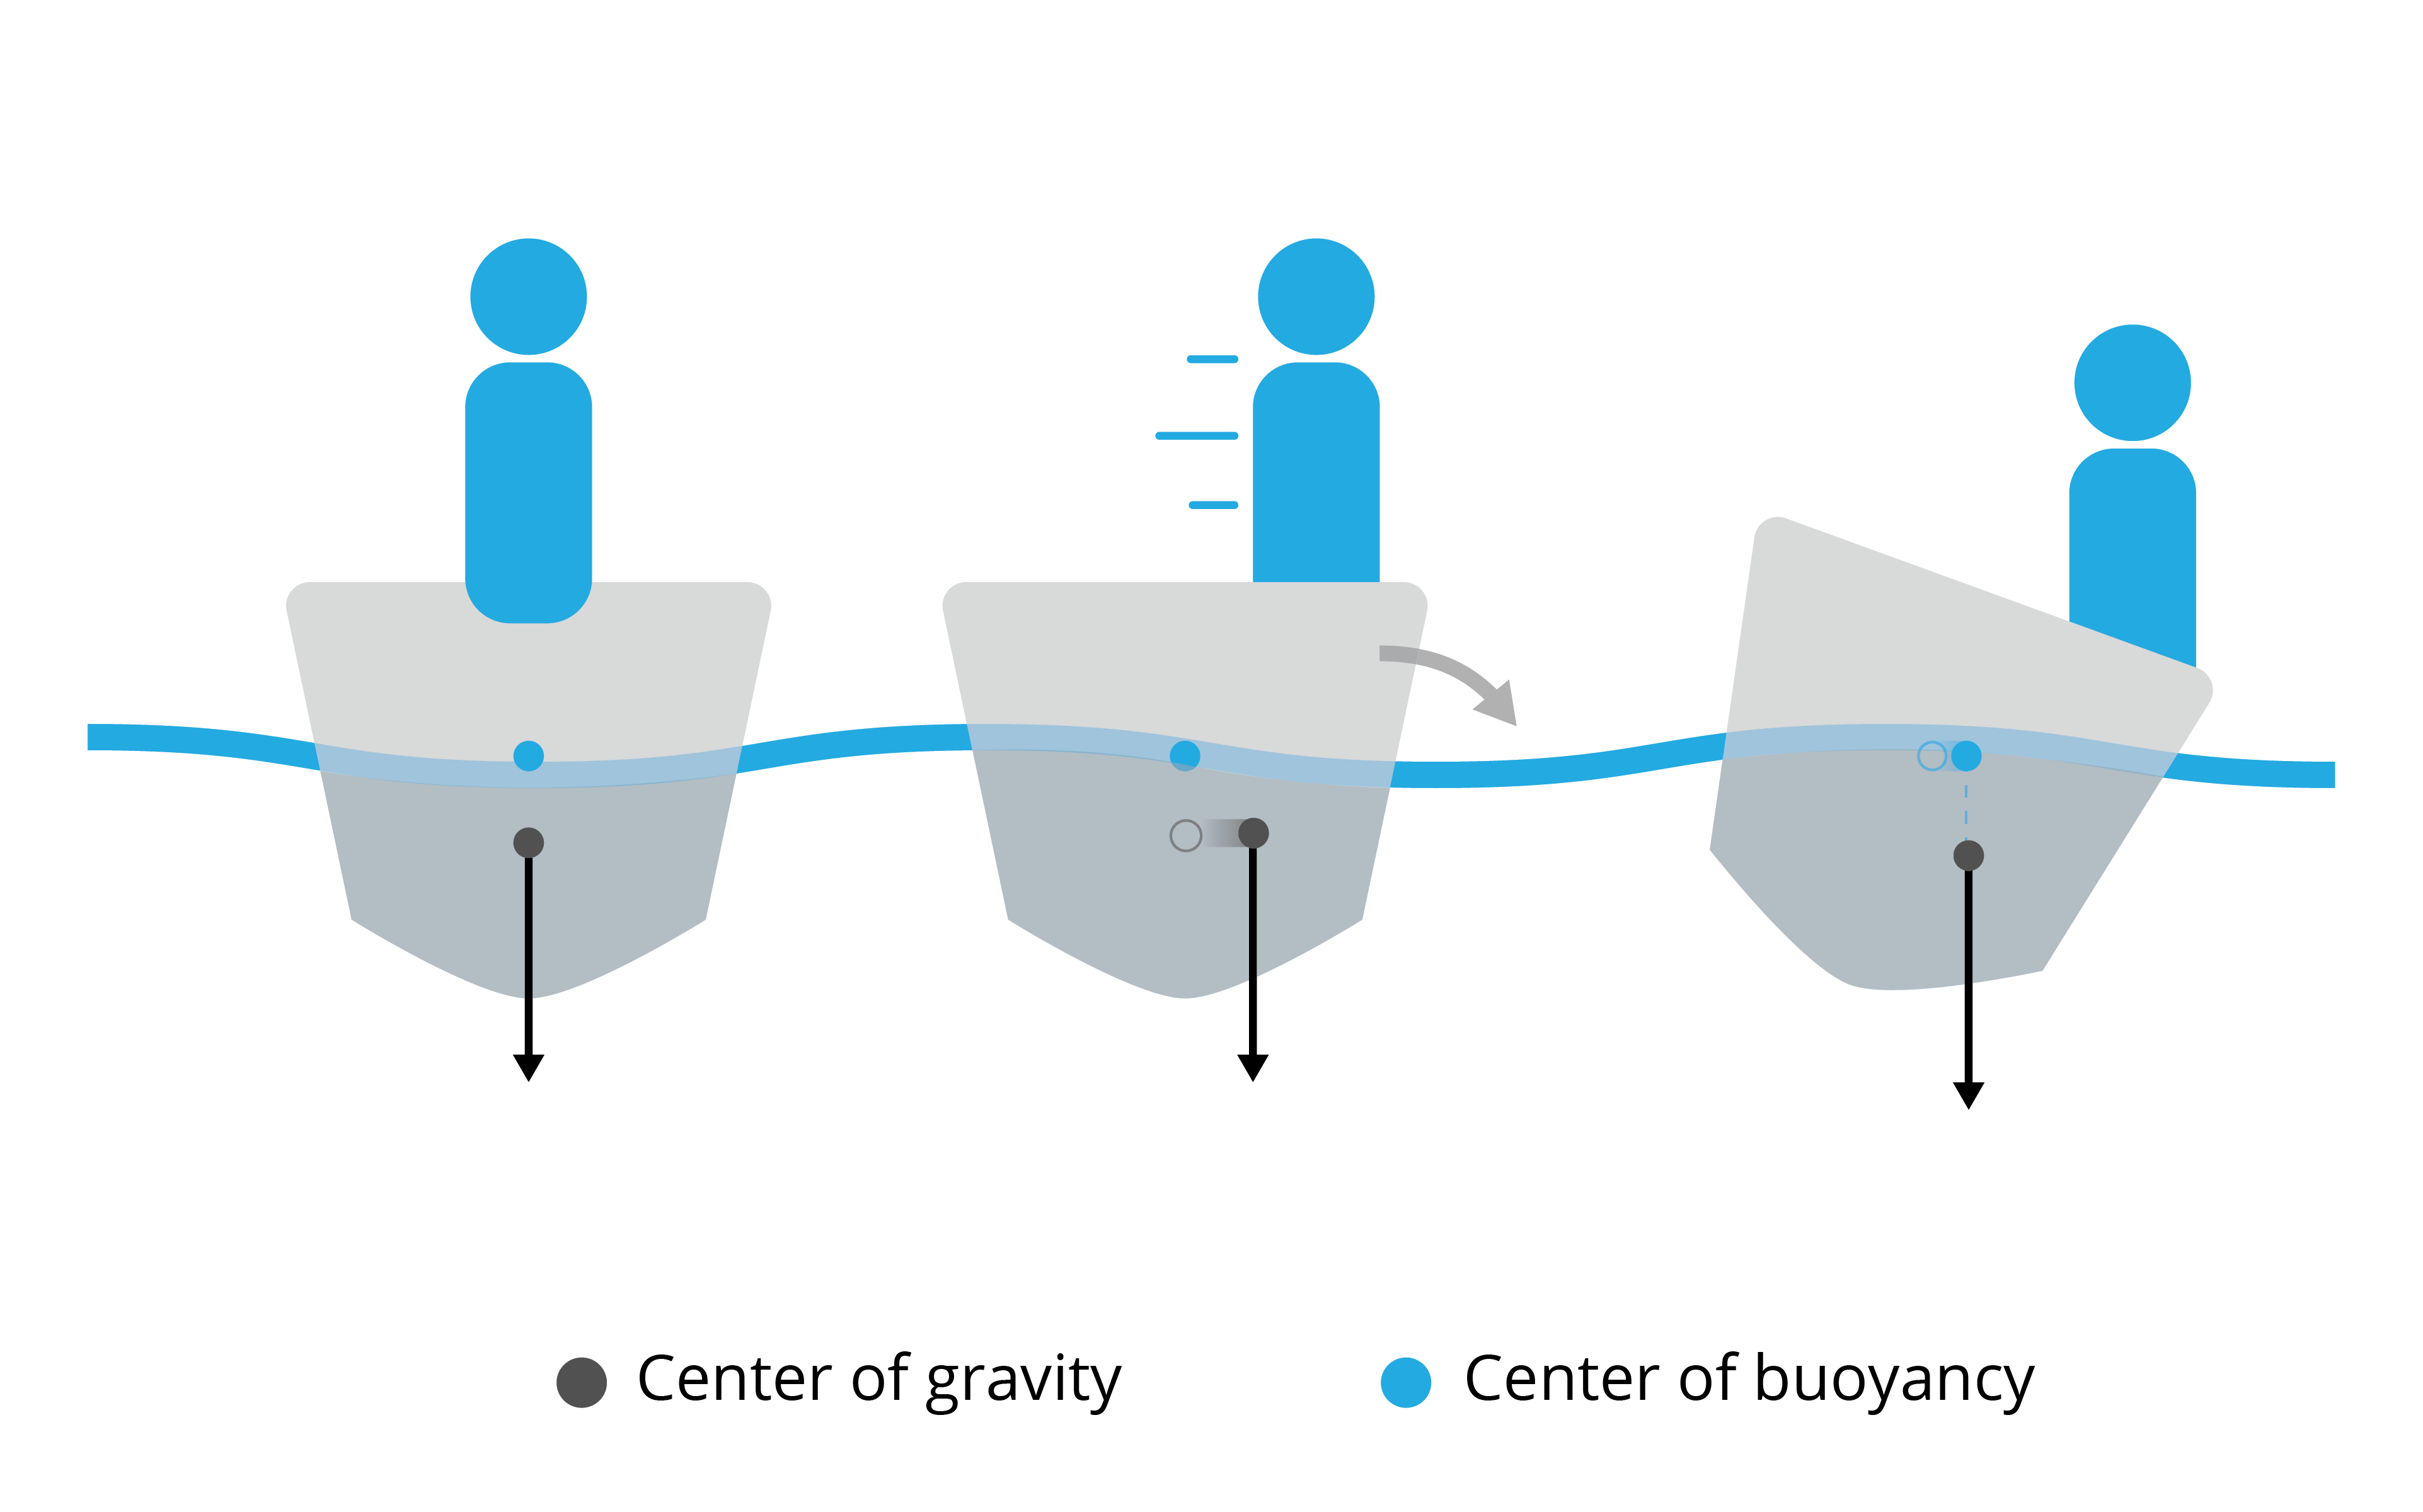
\includegraphics[width=.75\textwidth]{cgcm.png}

\end{center}

\subsection{Center of Lateral Resistance}

It isn't enough for a boat to float --- for a boat to be useful,  it must also be able to travel in a straight line.

Imagine that you are standing knee-deep in a lake next to a canoe.  If you push the front of the canoe away from you,  it will rotate --- the back end will actually
swing toward you. There is a point near the middle of the canoe where if you push it will not rotate in either direction --- the boat will just slide sideways.  This point is known as the \newterm{center of lateral resistance}\index{center of lateral resistance}.

The trick to making a boat travel in a straight line is to make sure that the line that contains the thrust vector passes through the center of lateral resistance.

An outboard motor allows you to direct the thrust vector. When the line of thrust passes the center of lateral resistance on the starboard side of the center of lateral resistance, the boat turns toward the port side.

\begin{center}
    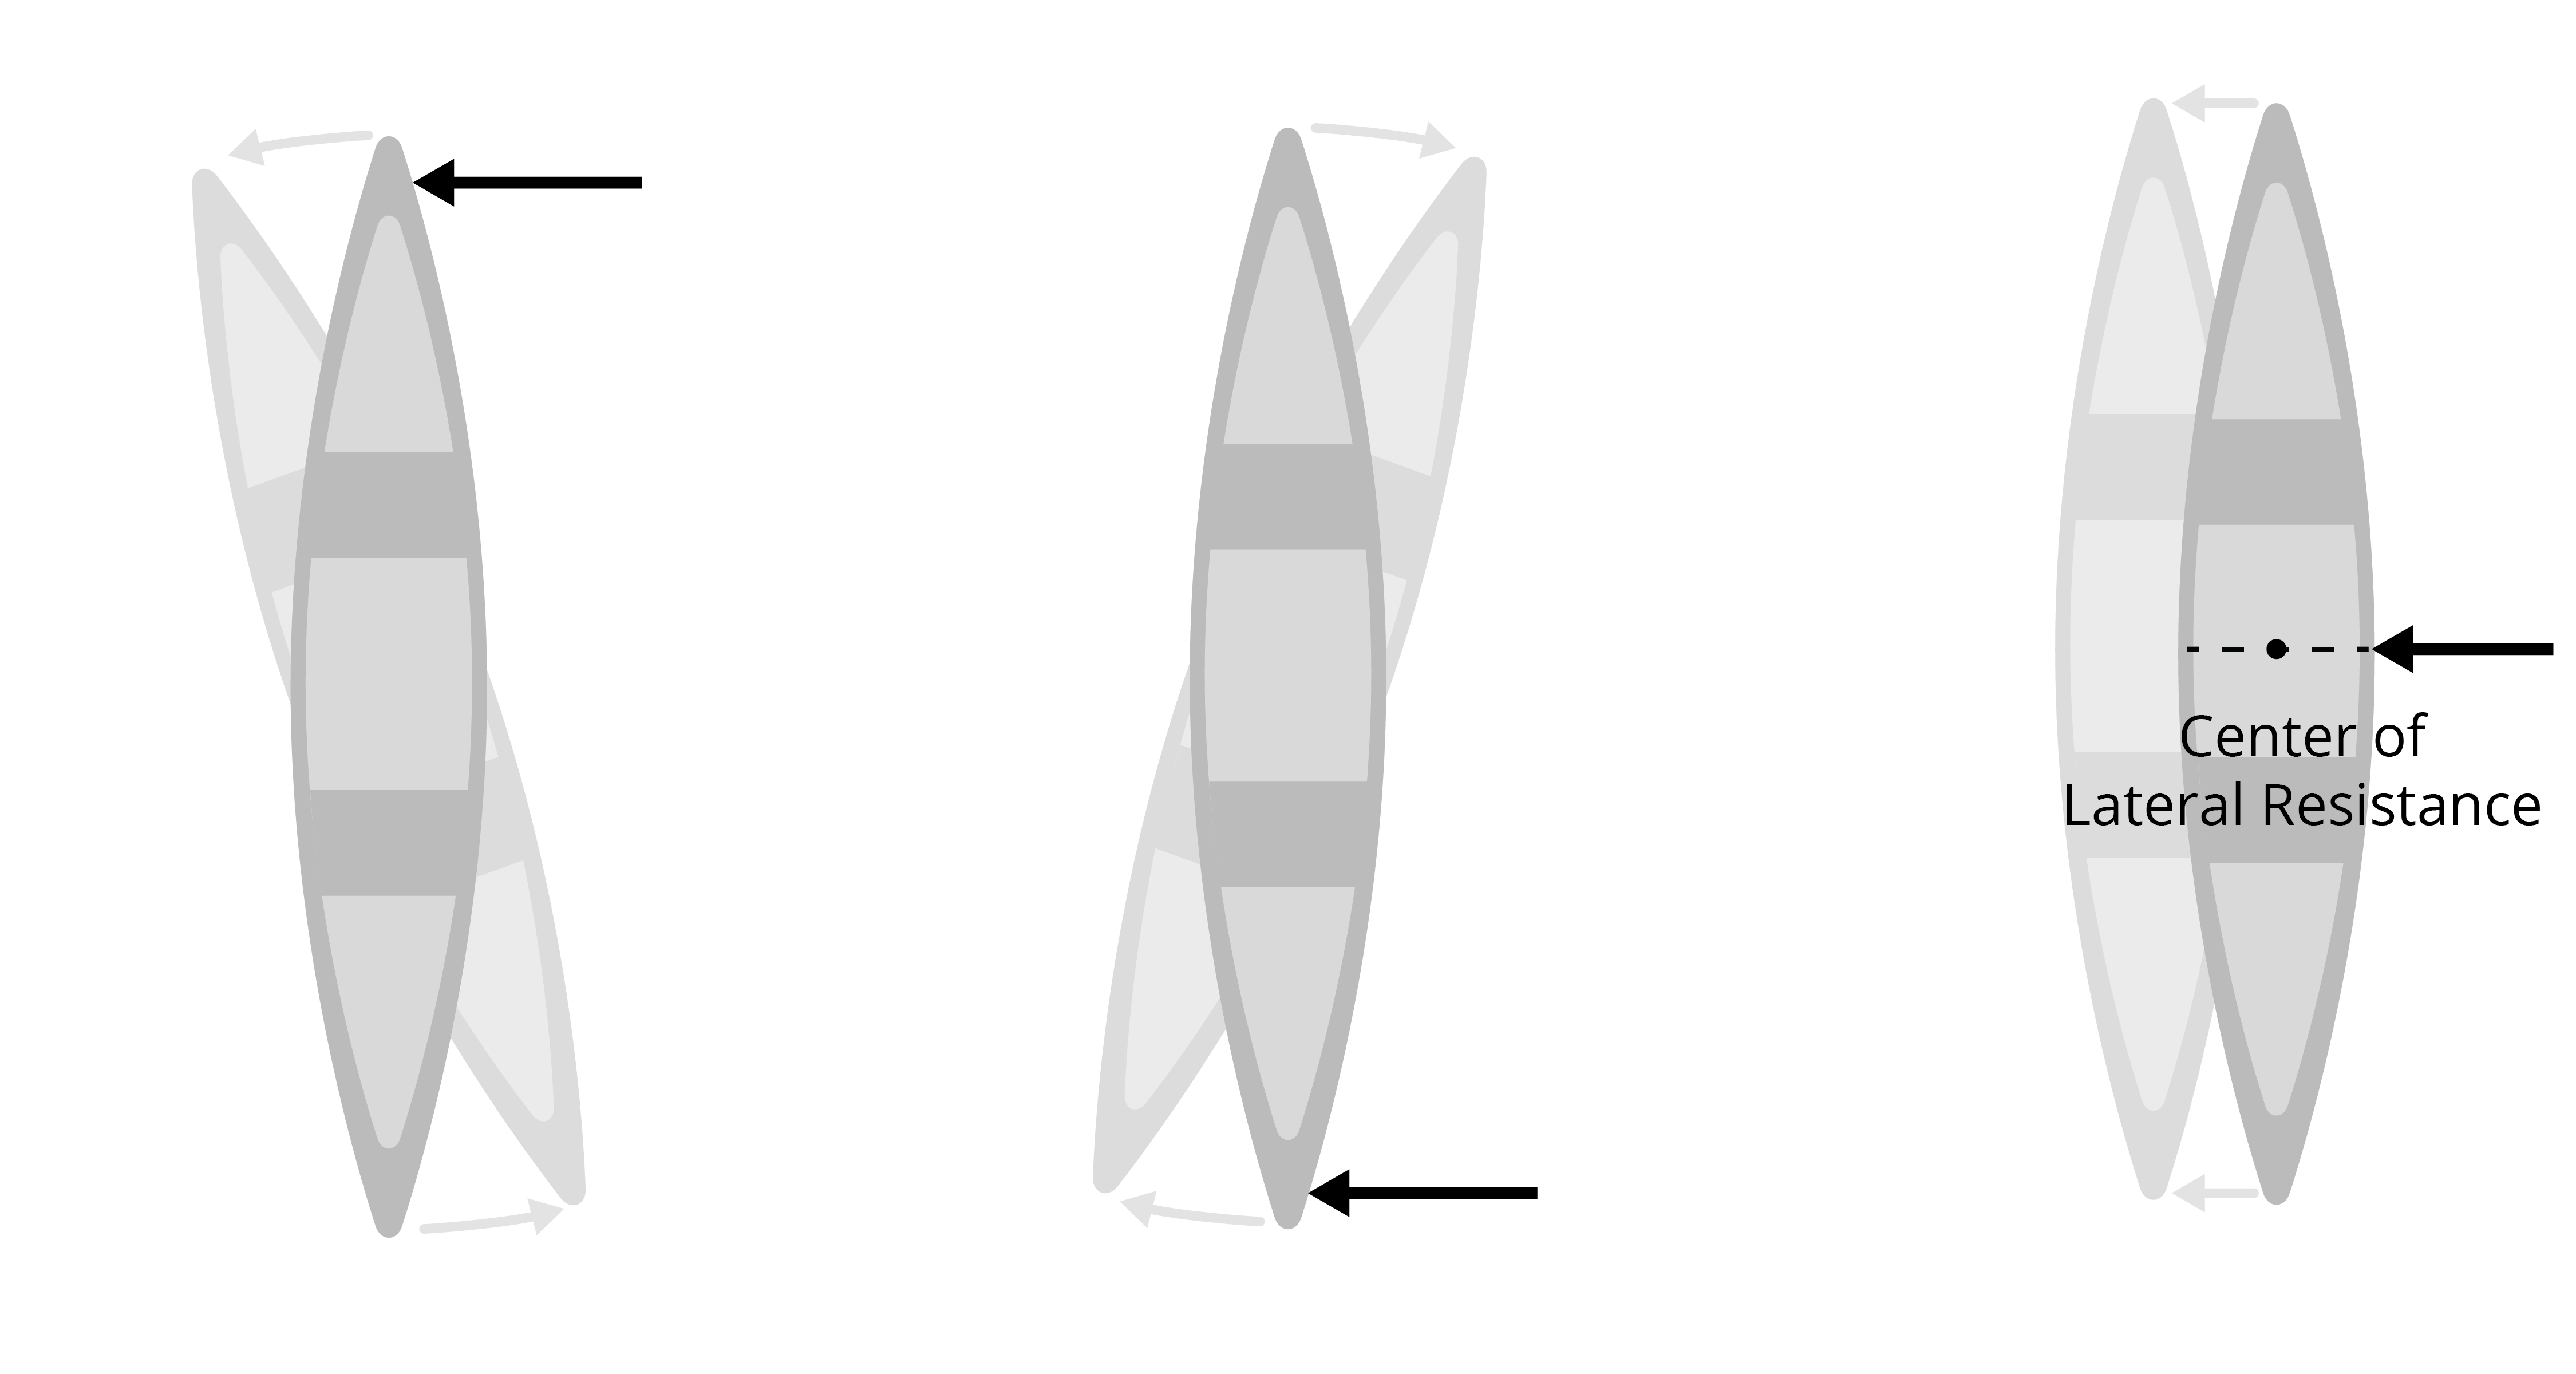
\includegraphics[width=.75\textwidth]{lateralResistance.png}

\end{center}

\subsection{Steering with a Rudder}
\index{rudder}
While outboard motors and airboats let you direct the thrust vector,  most boats have a \newterm{rudder}.  The rudder is a blade on a pivot near the back of
the boat. The angle of the rudder can be adjusted so that water rushing past it gets pushed to one side or the other.

According to Newton's third law,  when the water gets pushed to the left,  the back of the boat gets pushed (with the same force) to the right.  This causes the boat to rotate around its center of lateral resistance.

Note that a rudder only works when the boat is passing through the water.

\begin{center}
    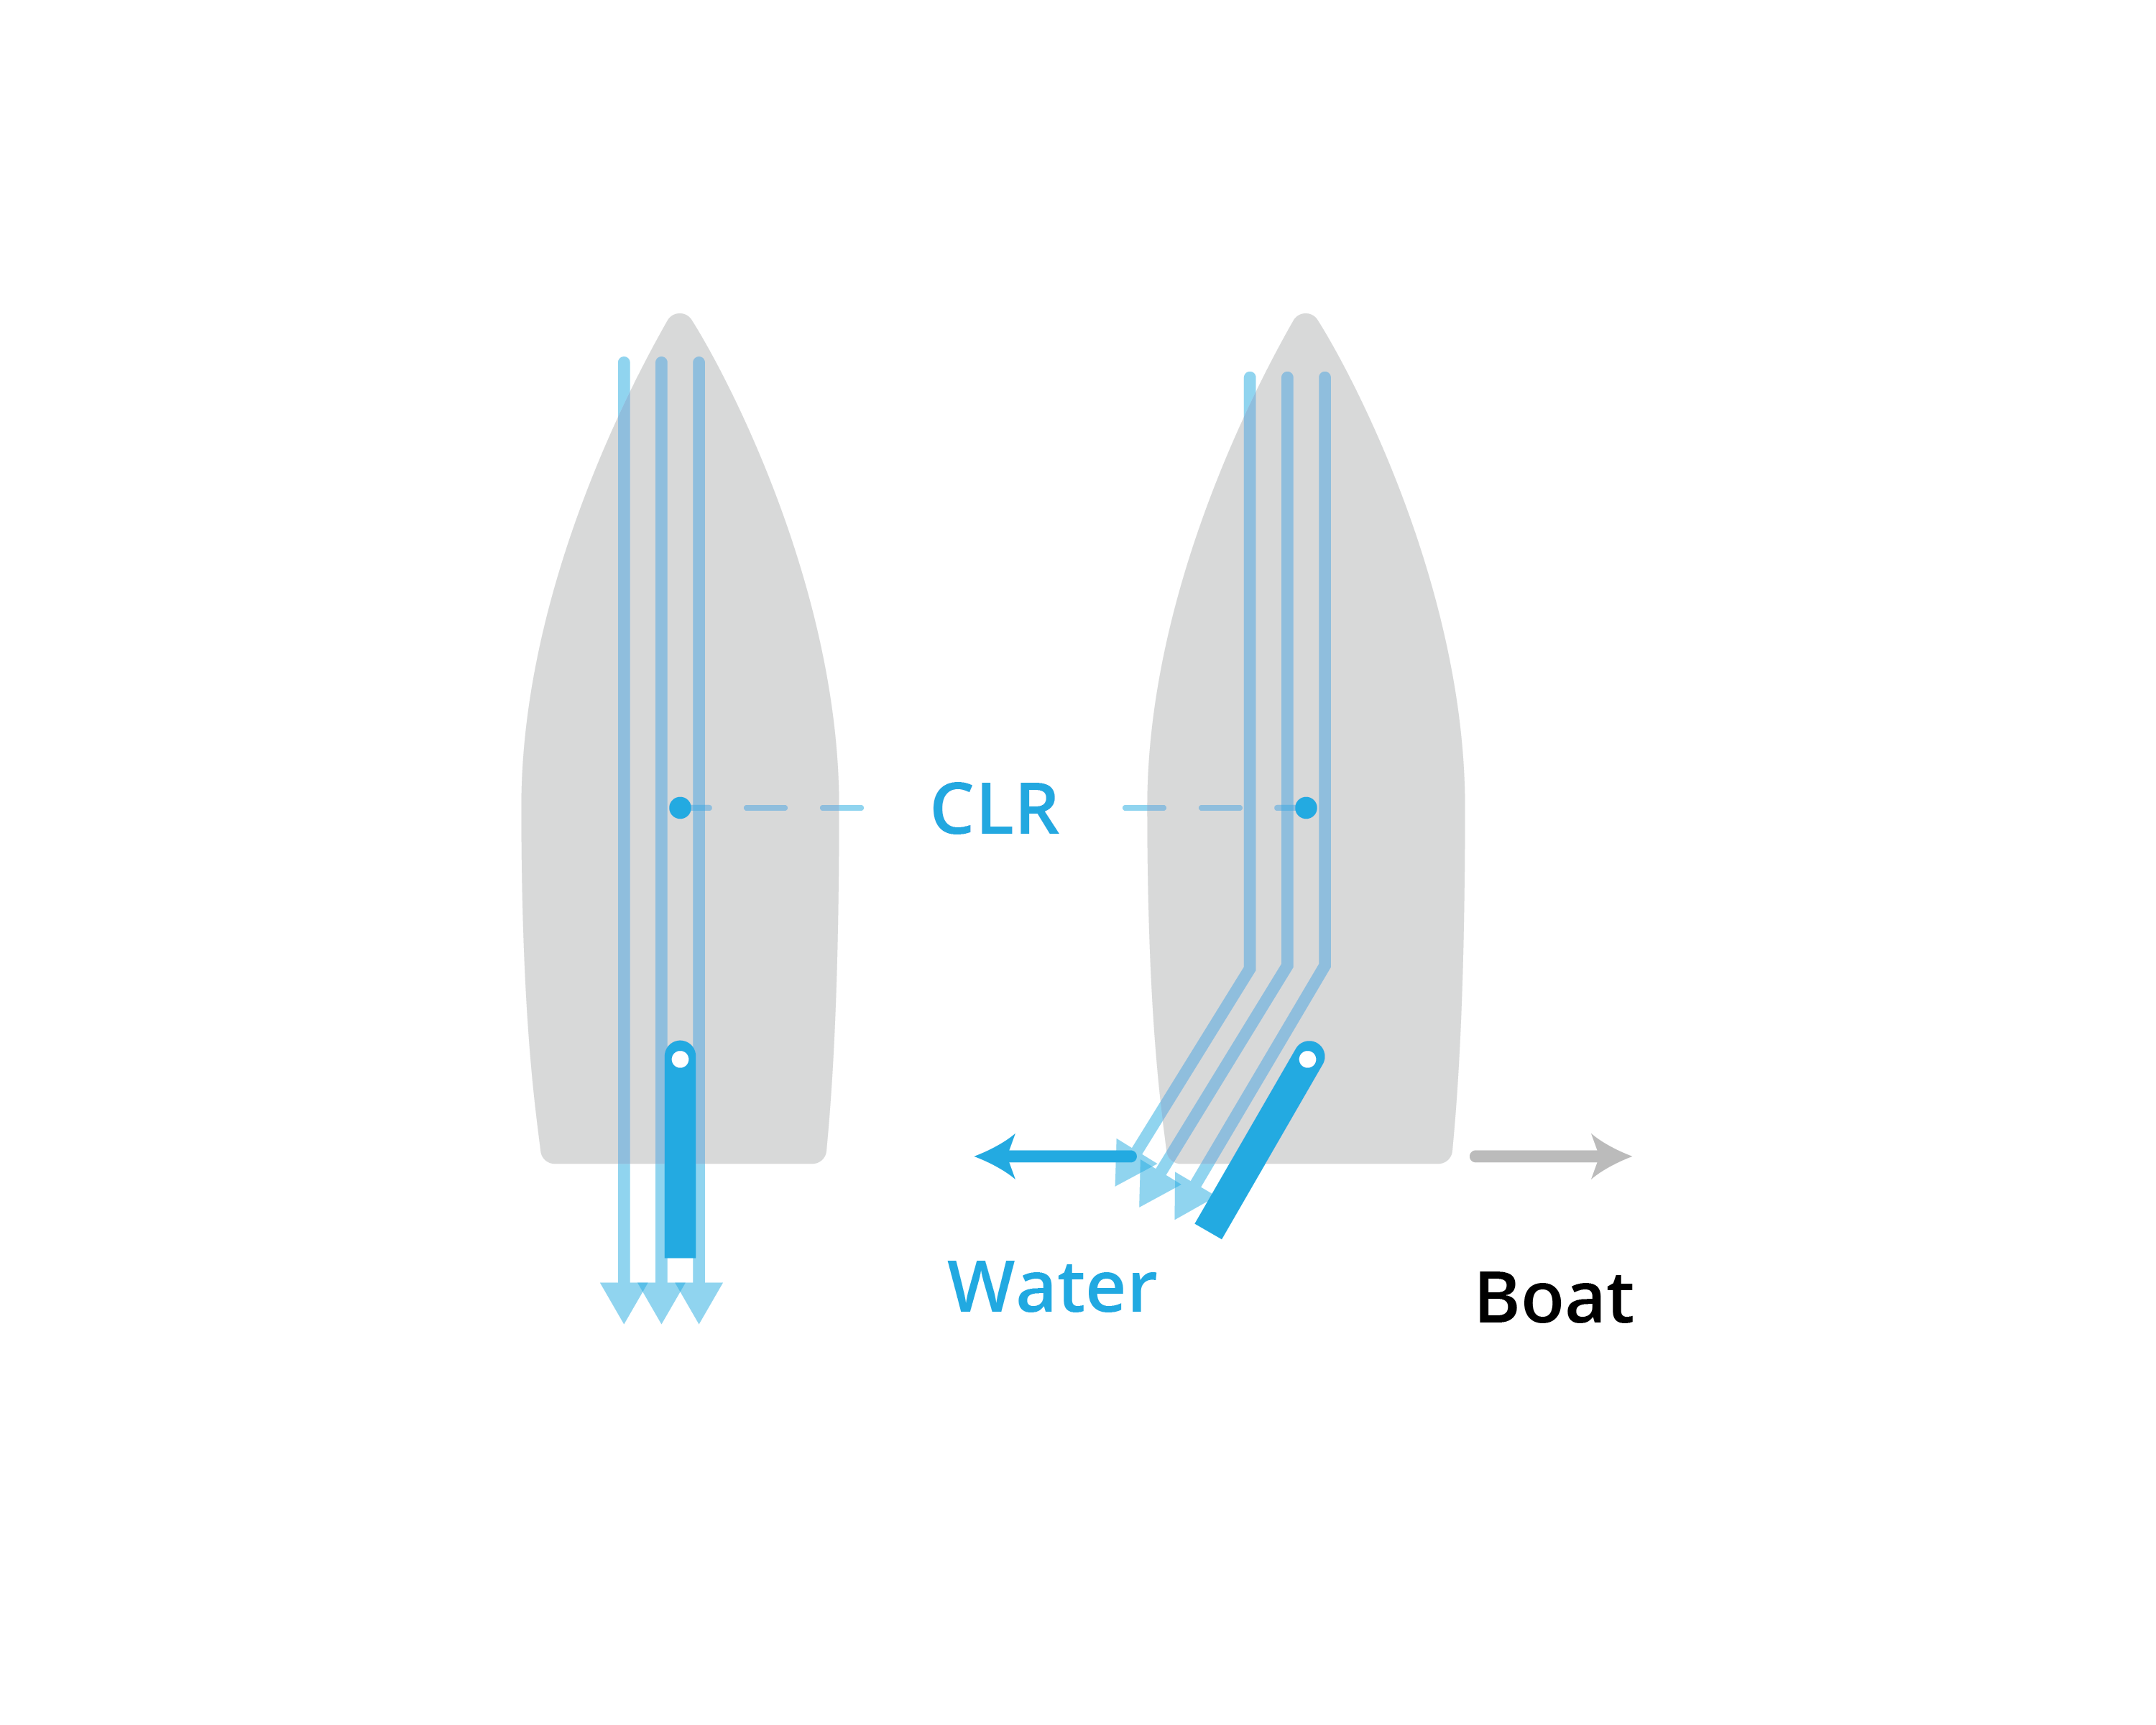
\includegraphics[width=.75\textwidth]{rudder.png}

\end{center}

\subsection{Boat Length and Resistance}

FIXME: Write about wave length,  boat length, and Froude number.


\section{Sailboats}
Imagine that you have a canoe, and you are about to paddle from one island to another that is directly east of where you are standing. There
is also a steady wind coming from the west, and you have a big piece of plywood.  You might be inspired to use it as a sail.

This situation is the most simple form of sailing: Wind comes from behind the boat and hits the sail which generates a force that pushes the
boat in the direction of the wind.

The sail has two sides:  The \newterm{windward} side is the one that is getting hit with the wind. The \newterm{leeward} side is the side away from the wind.
\index{windward}
\index{leeward}
\begin{center}
    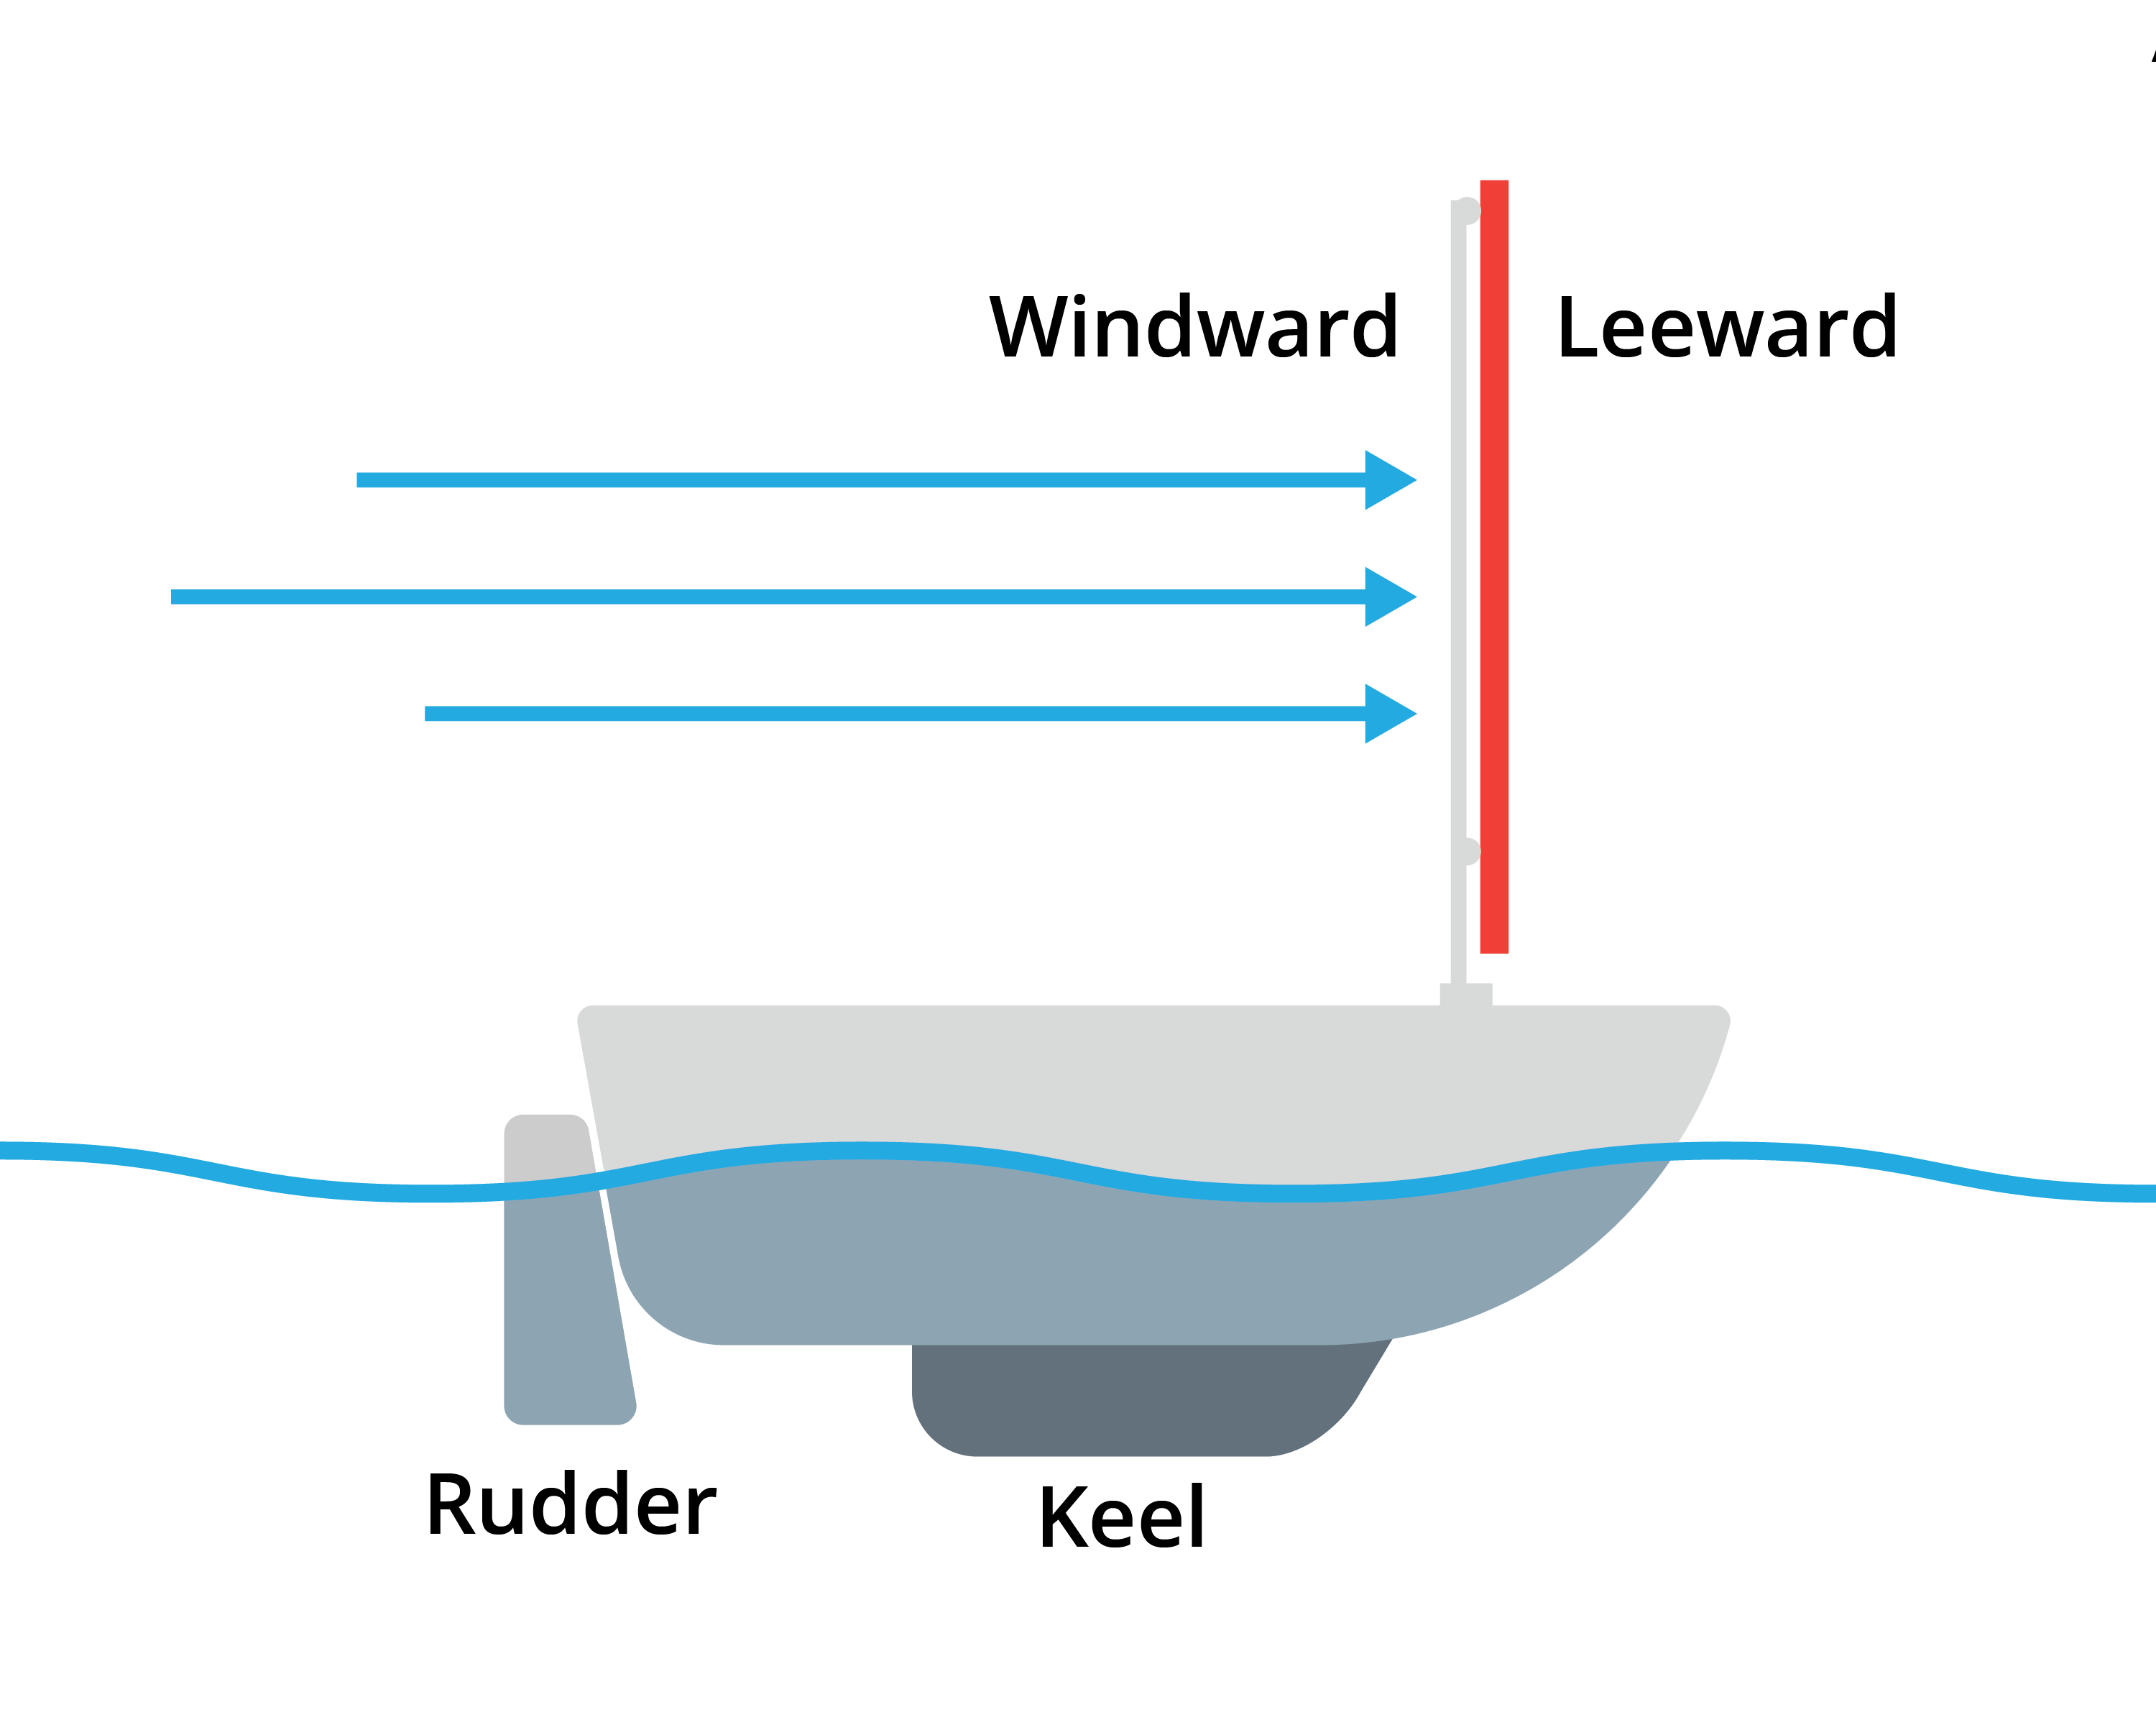
\includegraphics[width=.75\textwidth]{plywood.png}

\end{center}

\subsection{Magnitude of the Wind Force}

The first natural question is: How much force will I have pushing my canoe through the water?
\index{windward}
\begin{mdframed}[style=important, frametitle={Wind Force}]

When the sail is perpendicular to the wind,  the force of the wind on the sail in newtons ($F_w$) will be given by:

$$F_w = A \frac{d v^2}{2}$$

where $A$ is the area of the sail in square meters  $d$ is the density of the gas in kg per cubic meter, and $v$ is the wind speed in meters per second.

For air at STP,  $d$ is about 1.225 kg per cubic meter.

We call $\frac{d v^2}{2}$  the \newterm{wind pressure}\index{wind pressure}.  This is the amount of pressure that the windward side of plywood is experiencing that is above the
 pressure that the leeward side of the plywood is experiencing.  (The leeward side might experience some turbulence,  but the pressure it is experiencing is
 approximately 1 atmosphere.)

\end{mdframed}

Let's say your canoe is standing still and the wind is 0.5 m/s.  This means the wind pressure is

$$P =  \frac{1.225 (0.5^2)}{2} =  0.153125 \text{ newtons per square meter}$$

Let's say your plywood sail is 2 meters tall and 1.5 meters wide.  What will be the force of the wind?

$$F_w  = A P = (3)(0.153125) \approx 0.46 \text{ newtons}$$

This is a very intuitive idea: There is a difference between the pressure on the windward side and the pressure on the leeward side, and the plywood experiences a force that pushes
the boat through the water.
%FIXME diagram here?


\subsection{Direction and Location of the Wind Force}

If there is low pressure on one side of the sail and high pressure on the other,  the force vector will be perpendicular to the sail.

Where is this force vector applied?  We can think of the force as being applied at the geometric center of the sail.  This is called \newterm{the center of effort}\index{center of effort}. In this case,  the center of effort is the exact center of the rectangular plywood.

The mast on a windsurfing board can be tilted from side to side.  When the center of effort is over the center of lateral resistance,  the board goes straight.
To steer, the sailor moves the mast to one side of the center of lateral resistance, which rotates the board.

\subsection{Beam Reach}
\index{running}
When you are sailing in the same direction as the wind, sailors say you are \newterm{running}.

\begin{center}
    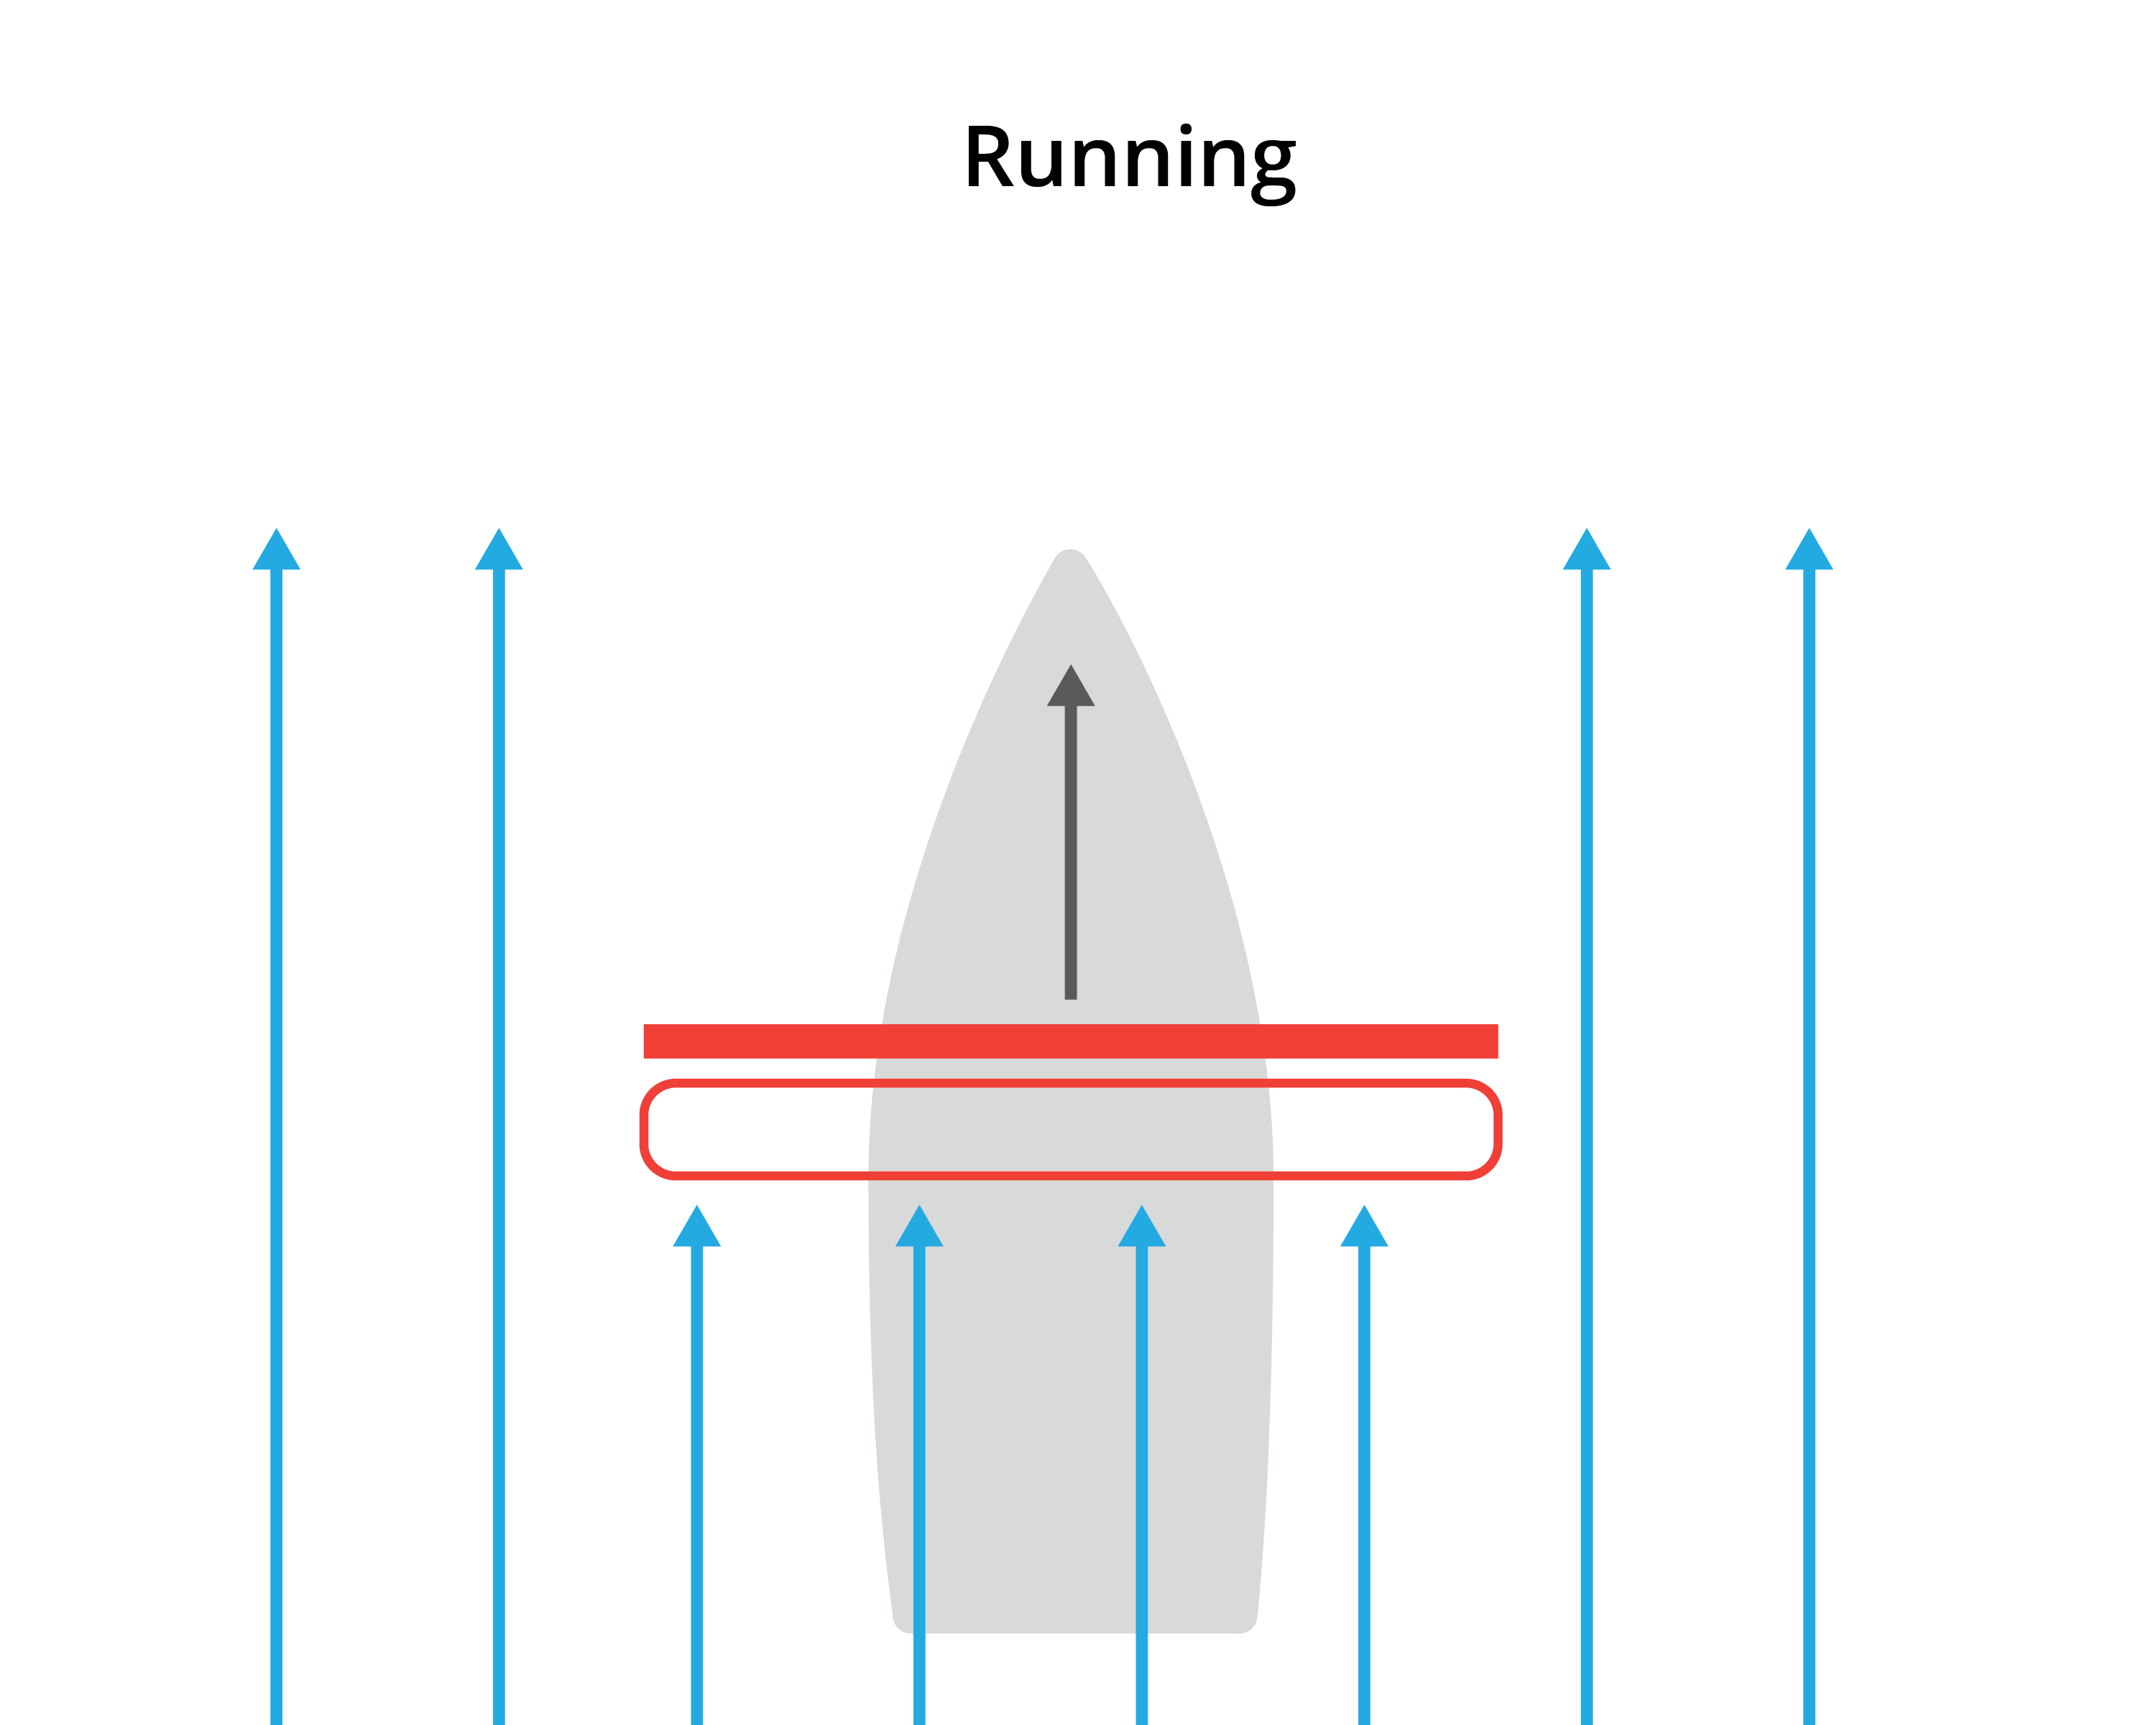
\includegraphics[width=.75\textwidth]{running.png}

\end{center}

What if you want to go east and the wind (still 0.5 m per second) is now coming from the south?  Sailing perpendicular to the wind is known as a \newterm{beam reach}\index{beam reach}.

\begin{center}
    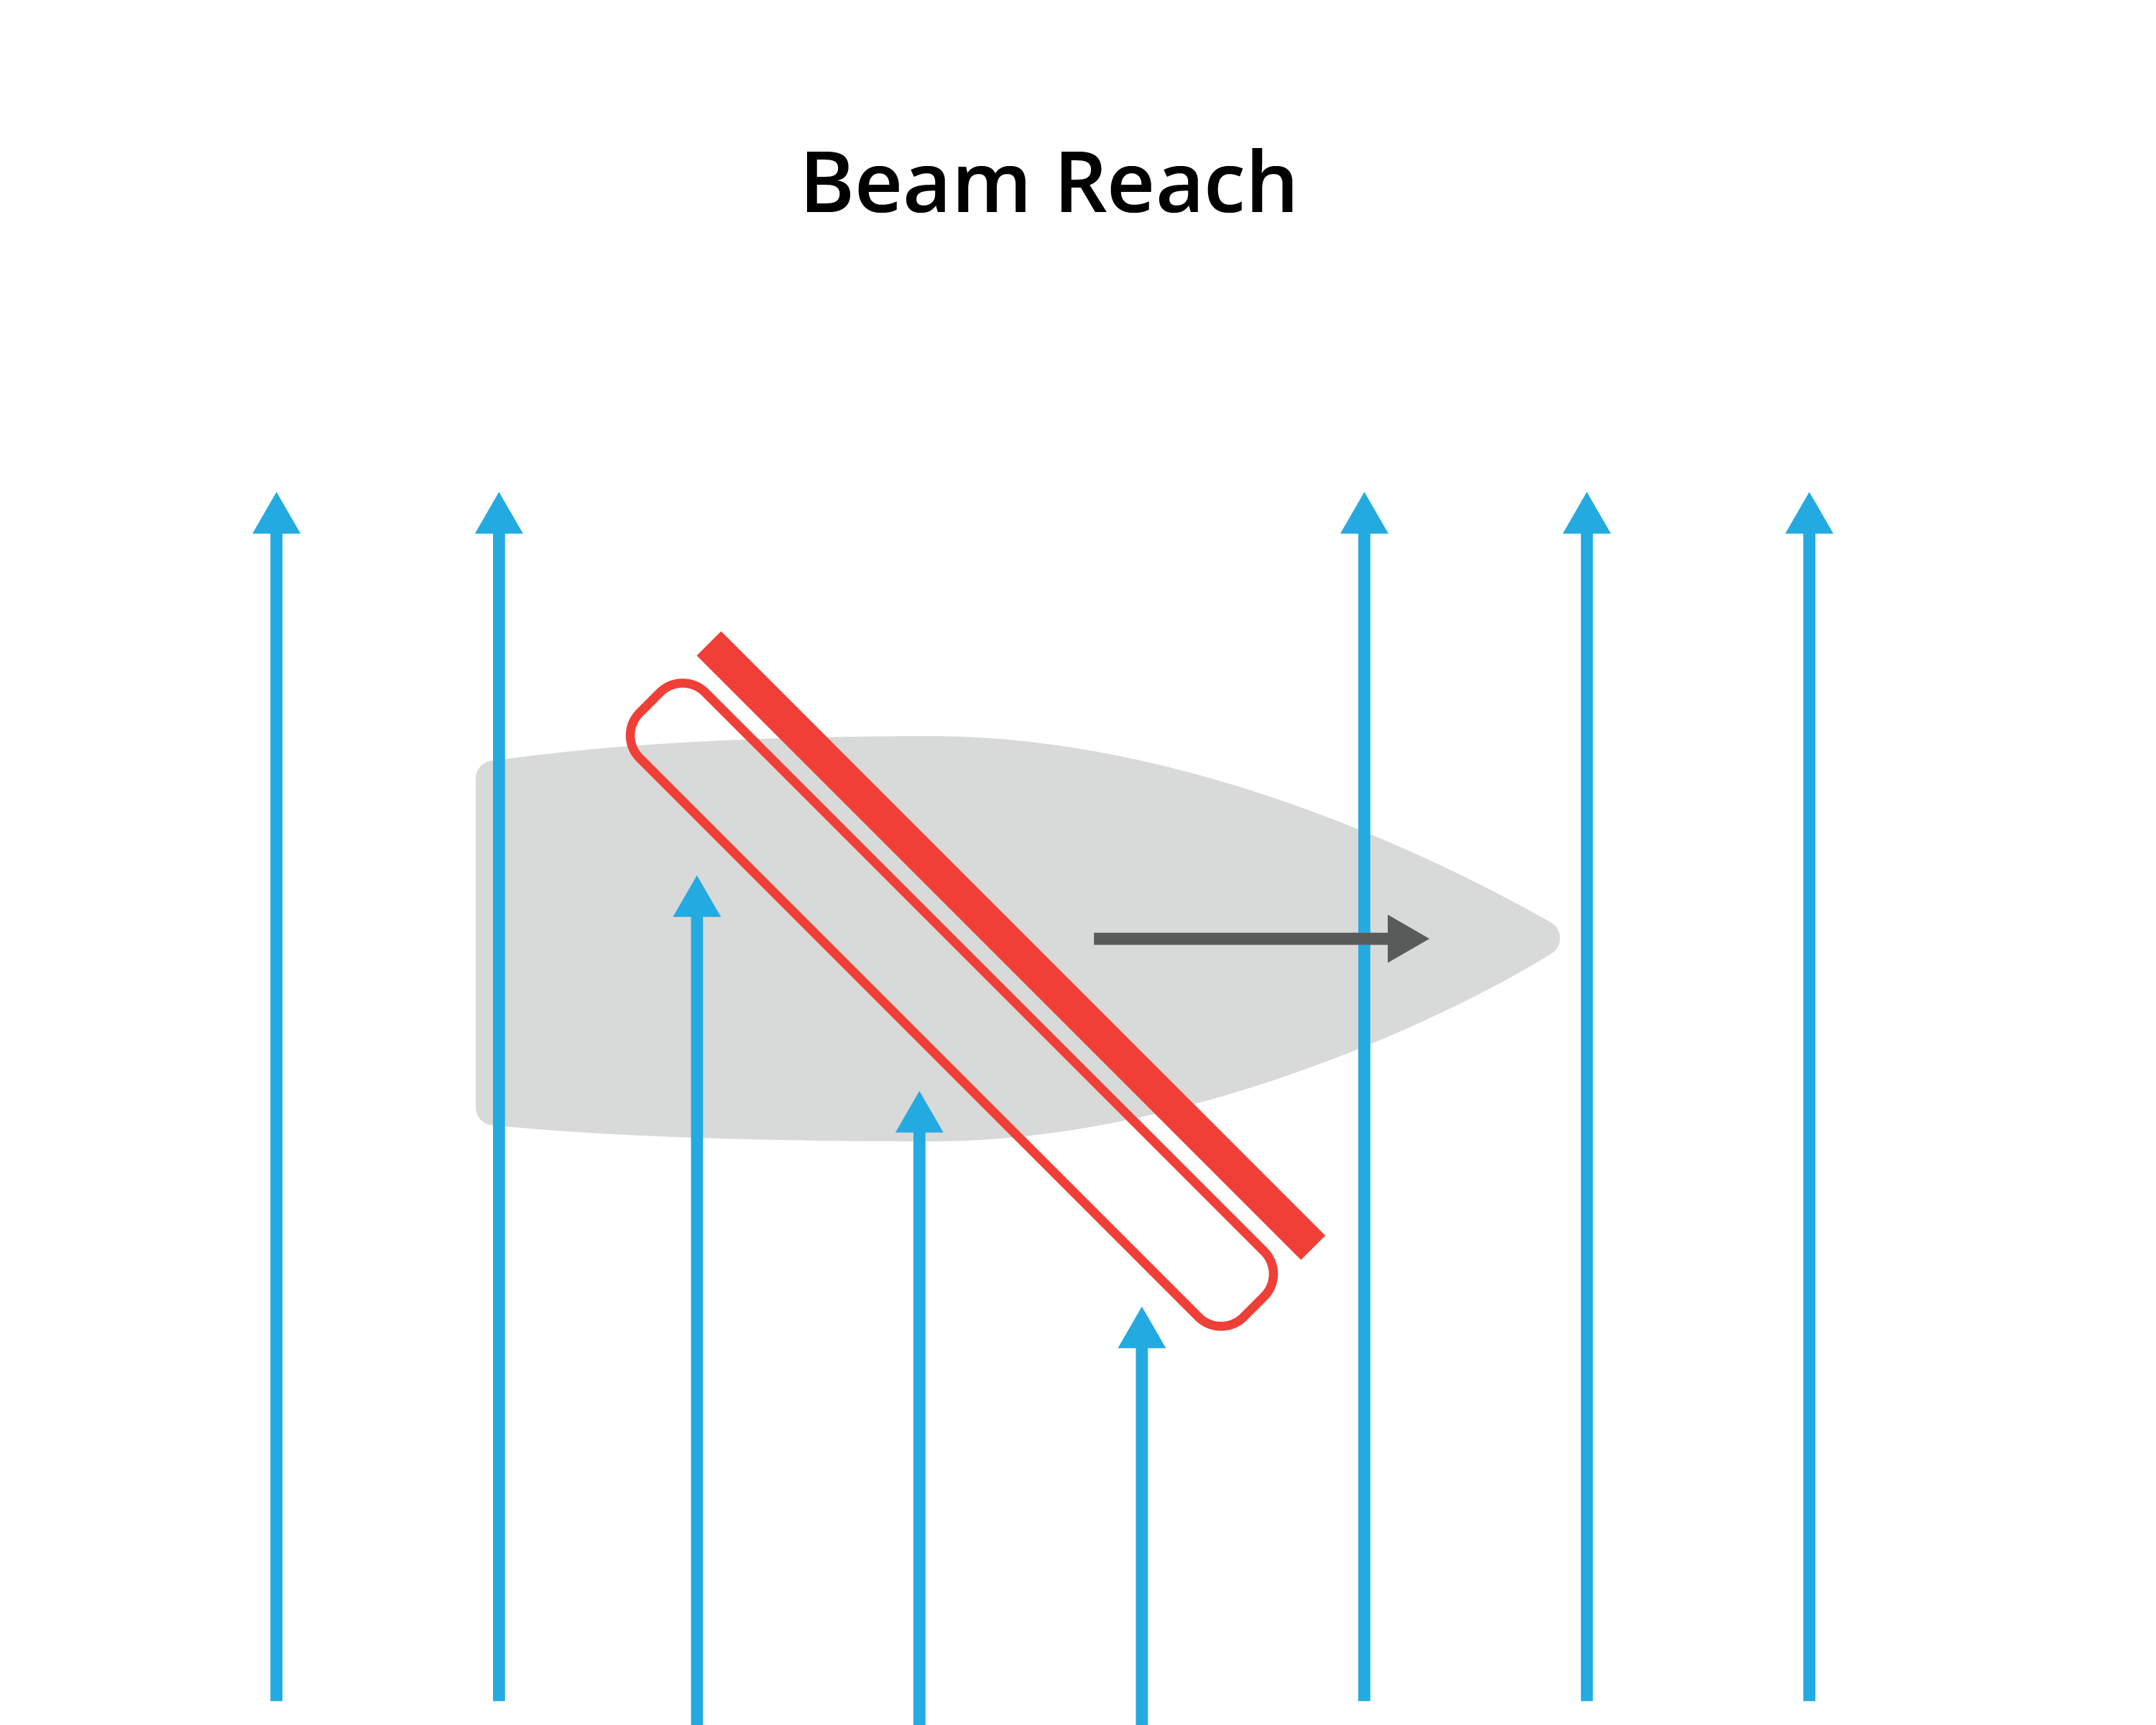
\includegraphics[width=.75\textwidth]{beamReach.png}

\end{center}

To do a beam reach,  instead of mounting the plywood perpendicular to the boats direction of travel,  you would mount it at a 45 degree angle. The wind pressure will build on the windward
side of the plywood,  and the plywood will experience a force pushing it at a $45^\circ$ angle to the boat.

We can think of this force as having two components:
\begin{itemize}
\item One component pushes the boat forward (Yay!)
\item One component pushes the boat sideways (Ugh!)
\end{itemize}
\begin{center}
    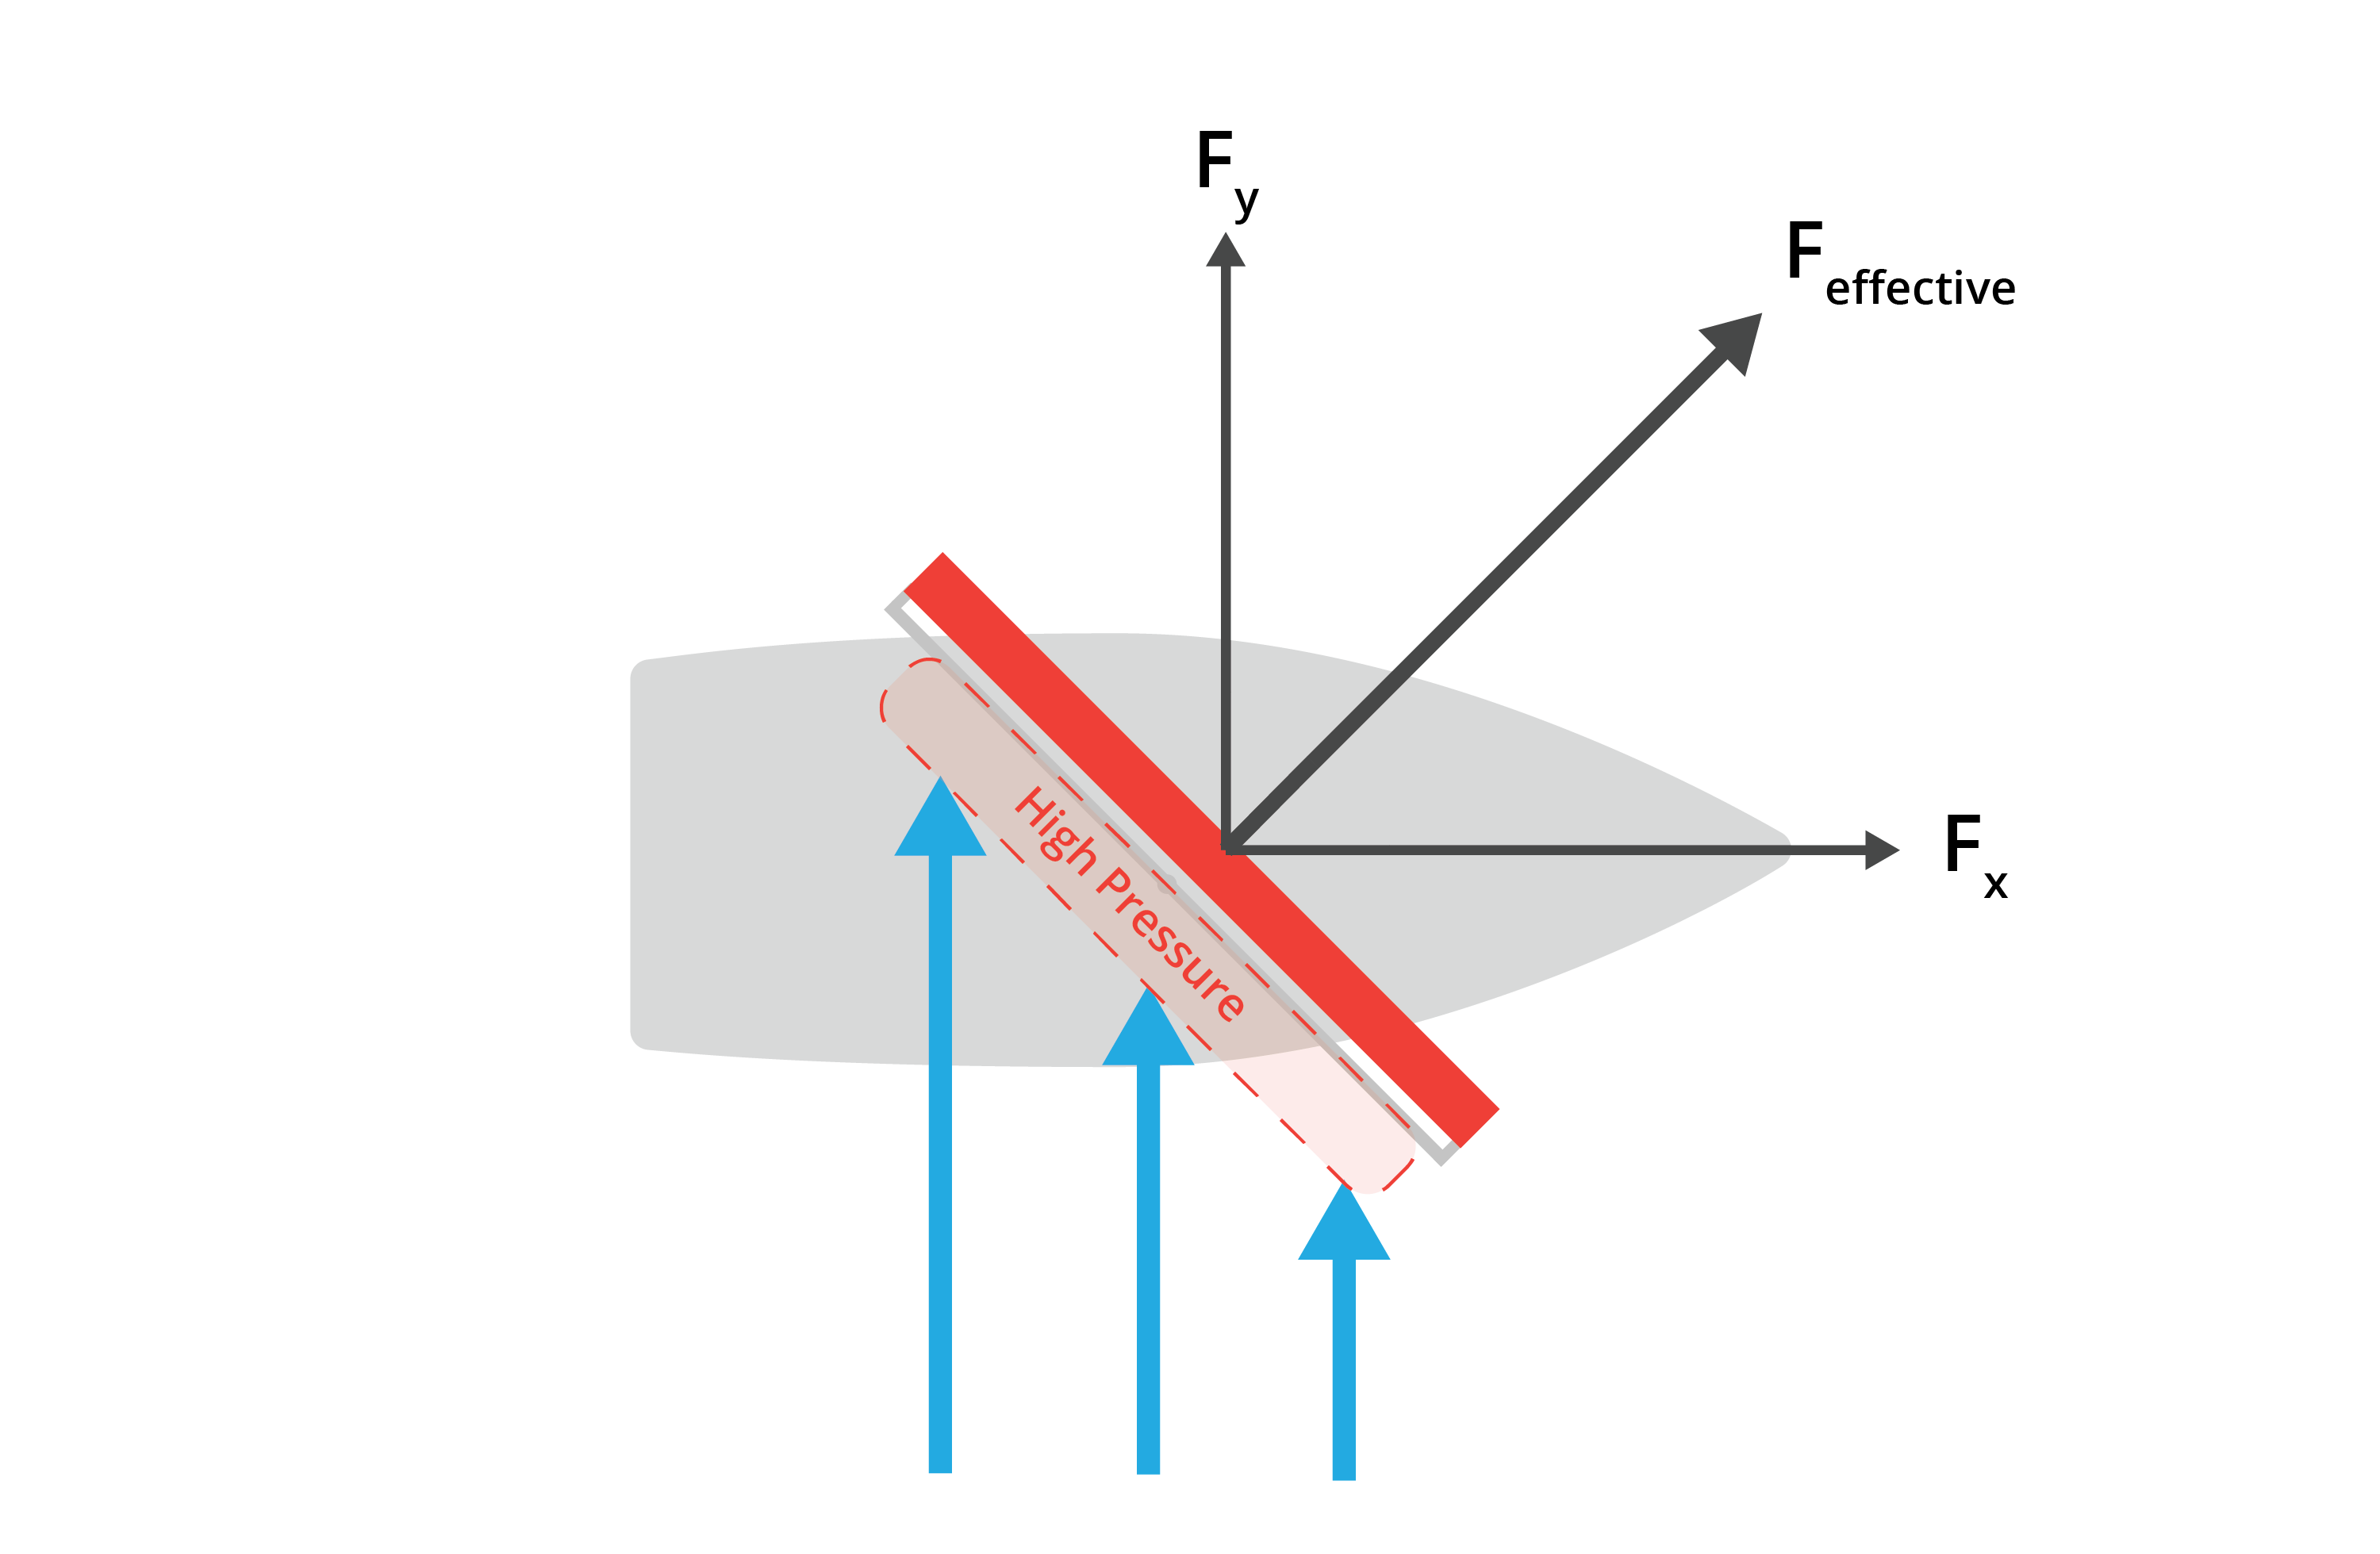
\includegraphics[width=.75\textwidth]{pressure.png}

\end{center}
To minimize the effect of the sideways force,  sailboats typically have  a keel --- \index{keel}a long fin on its underside that slows its sideways sliding.

\begin{center}
    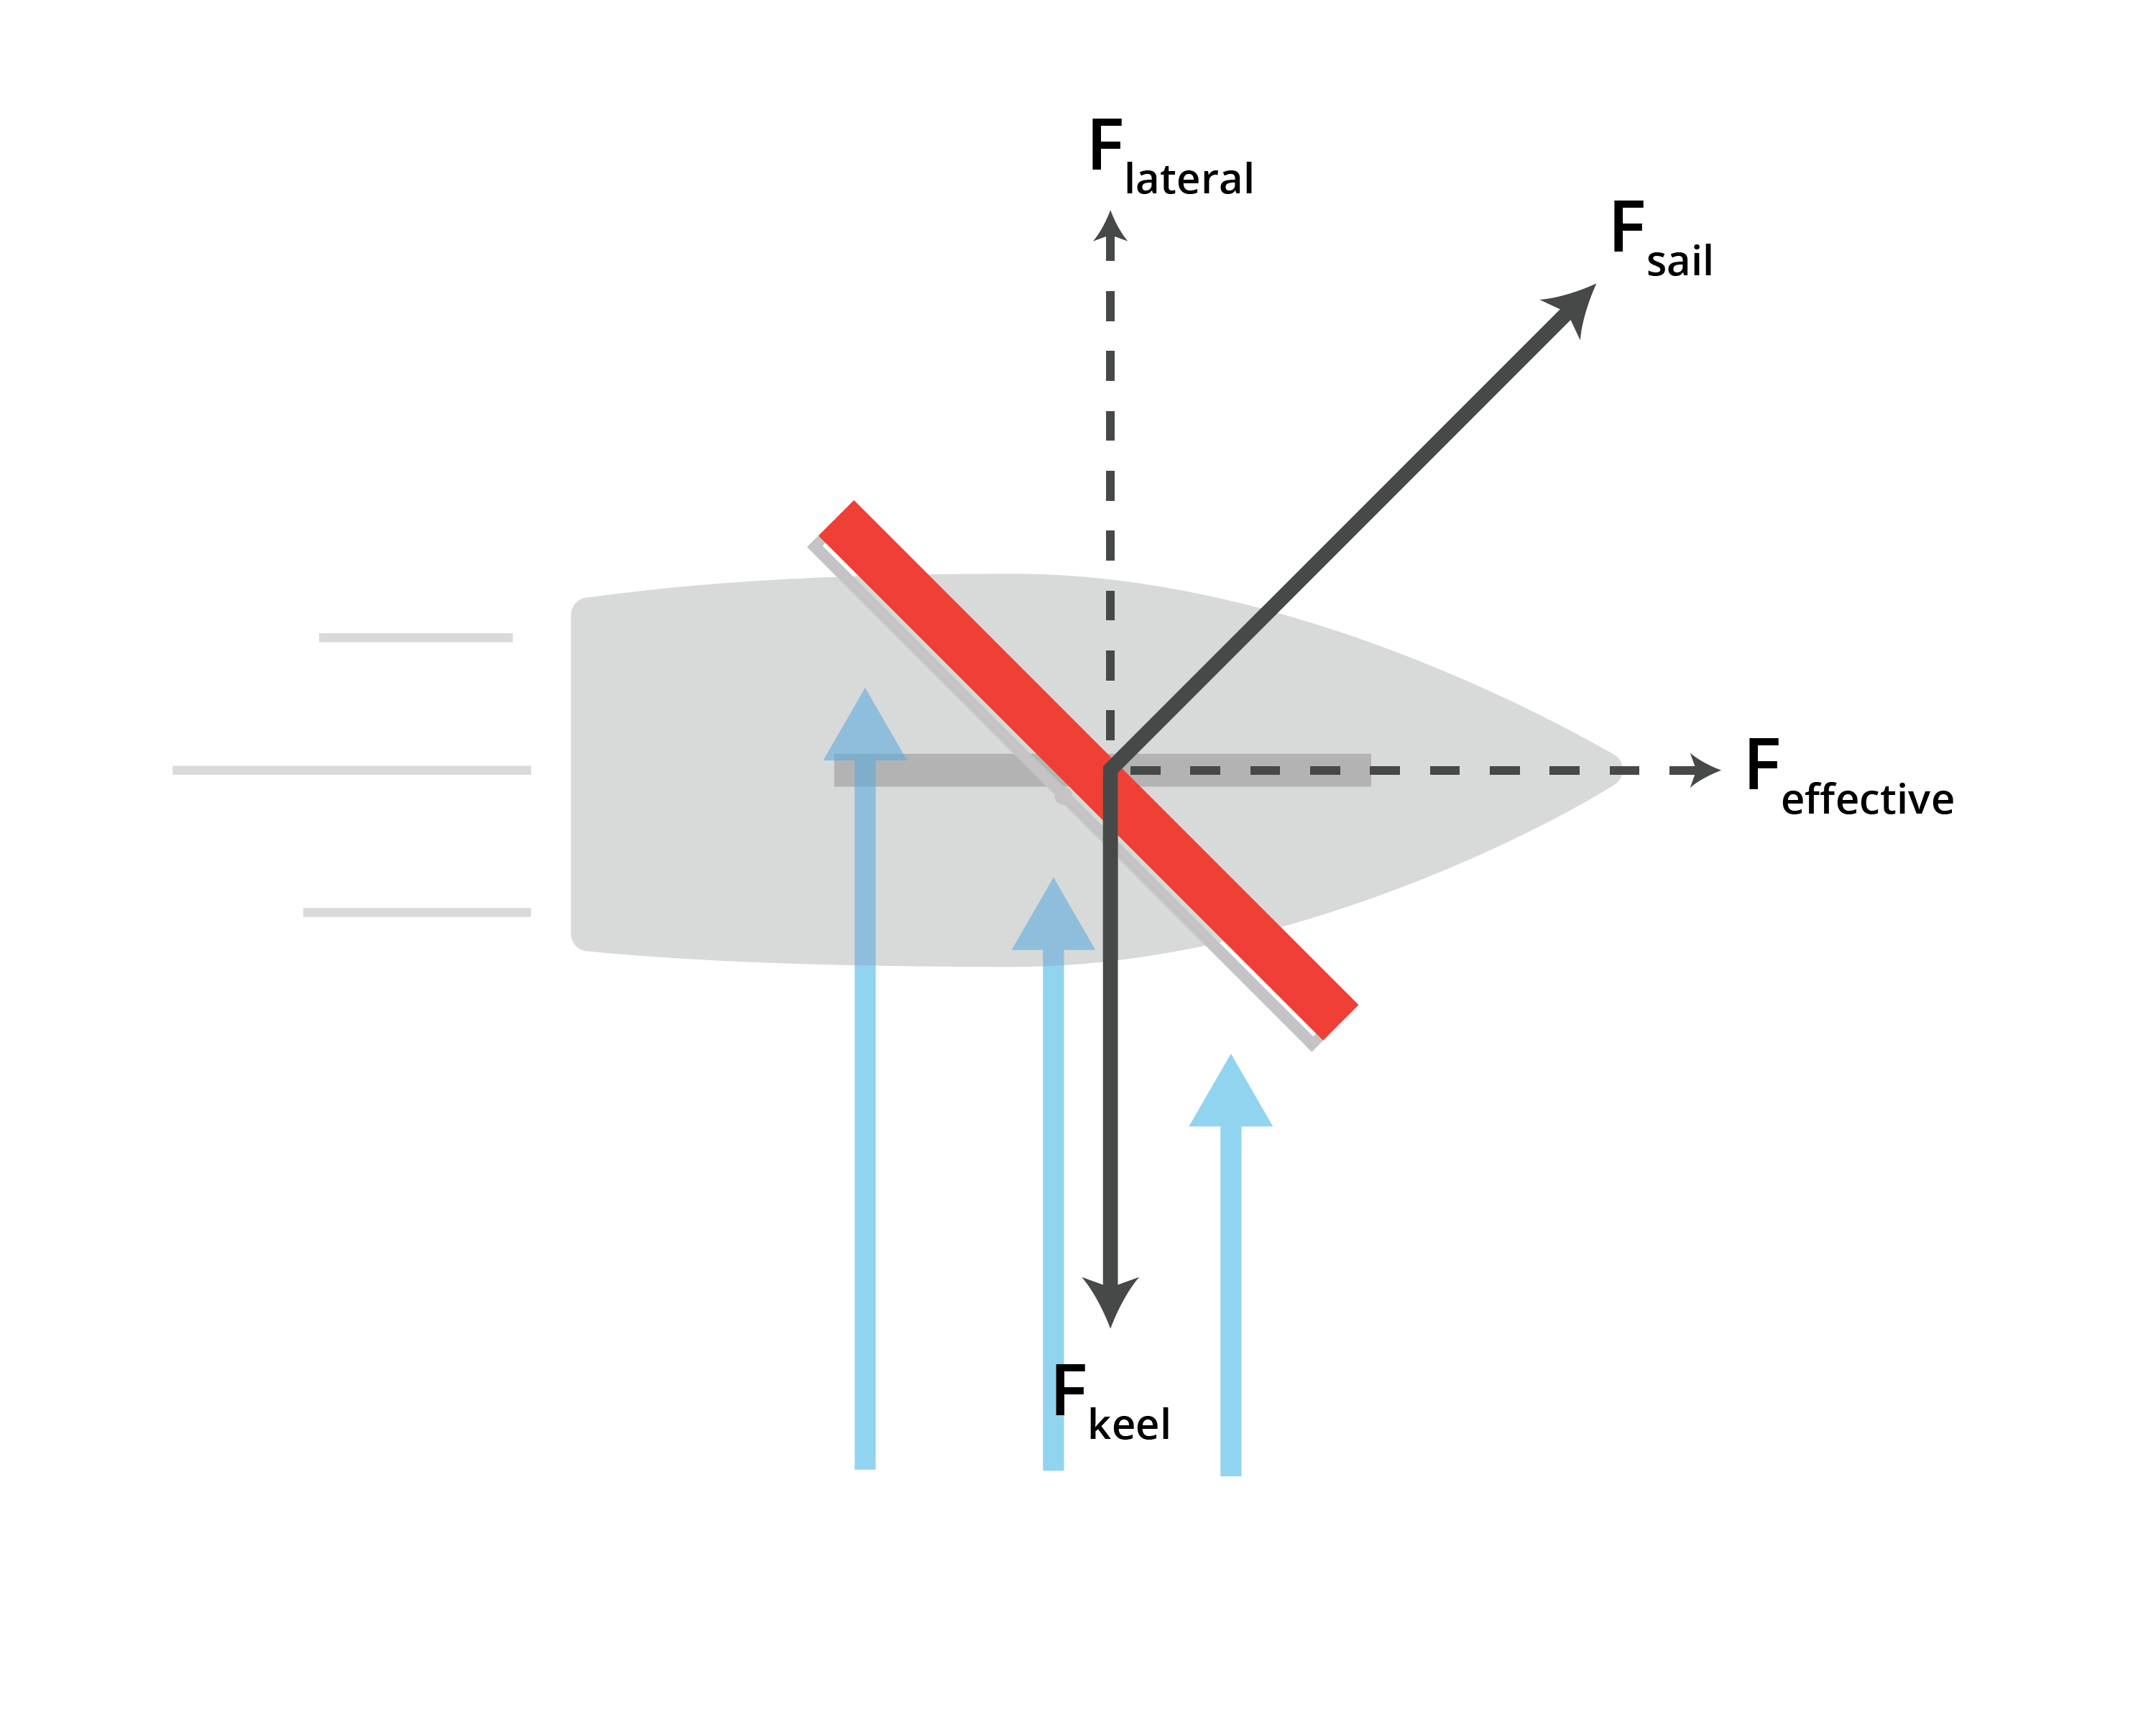
\includegraphics[width=.75\textwidth]{pressure2.png}

\end{center}

Notice also that the "wind shadow" of the plywood is smaller when it is at a $45^\circ$ angle to the wind.  How much smaller?  The effective area of your plywood has
gone from 3 square meters to $\frac{3}{\sqrt{2}} \approx 2.12$ square meters. This means the force generated will be smaller, and some of it will be wasted pushing the boat sideways.

If we assume that the wind pressure is still 0.153125 newtons per square meter. The force on the plywood will be about

$$F_w = A P = \frac{3}{\sqrt{2}}(0.154125) \approx 0.325 \text{ newtons}$$

However, the direction of that force is not all in the direction you want to go, so the effective force is

$$F = F_w \frac{1}{\sqrt{2}} =  \frac{3}{2}(0.154125) = 0.2311875 \text{ newtons}$$

Notice that we got twice as much effective force when we were running with the wind as when we are on a beam reach.  However, any sailor will tell you that you can go much faster
on a beam reach than you can running. Why?
\index{apparent wind}
\index{actual wind}
\subsection{Apparent Wind}

When you are running,  you can never go faster than the wind.   As you go faster and faster,  the wind that the boat experience decreases. For example, if you are going 0.2 m/s in a wind
of 0.5 m/s,  you (and your sail) will only experience wind at 0.3 m/s. We call the wind as experienced by the boat
the \newterm{apparent wind}.  The wind as observed by a stationary observer is called the \newterm{actual wind}.

If you are running with the wind, as you approach the speed of the wind,  the force of that wind will decrease towards zero.

On a beam reach, as you go faster, the direction of the wind seems to change. If you are going 0.2 m/s east and the actual wind is 0.5 m/s from the south, the direction of the
apparent wind will seem to come from about 22 degrees east of true south.  The speed of the apparent wind will be about 0.54 m/s.

\subsection{Close Reach}

What if you want to go east,  and the wind is coming from 40 degrees east of south?  This would mean that you were sailing just 50 degrees away from
straight into the wind. Is this possible?

If you put your sail at a 25 degree angle, you will still catch some wind and create some pressure on one side of the sail.  Most of the resulting force would be trying to push
your boat sideways,  but some of it would be in the direction you were trying to travel.

Picking an angle for your sail that creates high pressure that makes a desirable force is known as the "angle of attack".

This is a result does not feel intuitive. A boat can sail into the wind!? The boat can't sail directly into the wind -- with each degree that the boat gets closer
to straight into the wind,  the force pushing it forward decreases and the force pushing it back increases. However,  most boats can get within 45\% if they have a well-shaped sail.

\subsection{Shaping the Sail}

Most of the power of the wind can be captured with a piece of flat plywood.  The wind hits it and creates a high pressure on the windward side. What about the other side of the plywood?

It turns out that if we can get the wind to travel smoothly over the back side of the plywood,   the pressure on that side will be a little lower than if we had turbulence there.   (We are not going
to go too deeply into why. If you want to learn more, look up the Coanda effect.)

For example, if we were on a close reach, the very best sail we could have would gently pull the wind along its backside.  It would look like this:

\begin{center}
    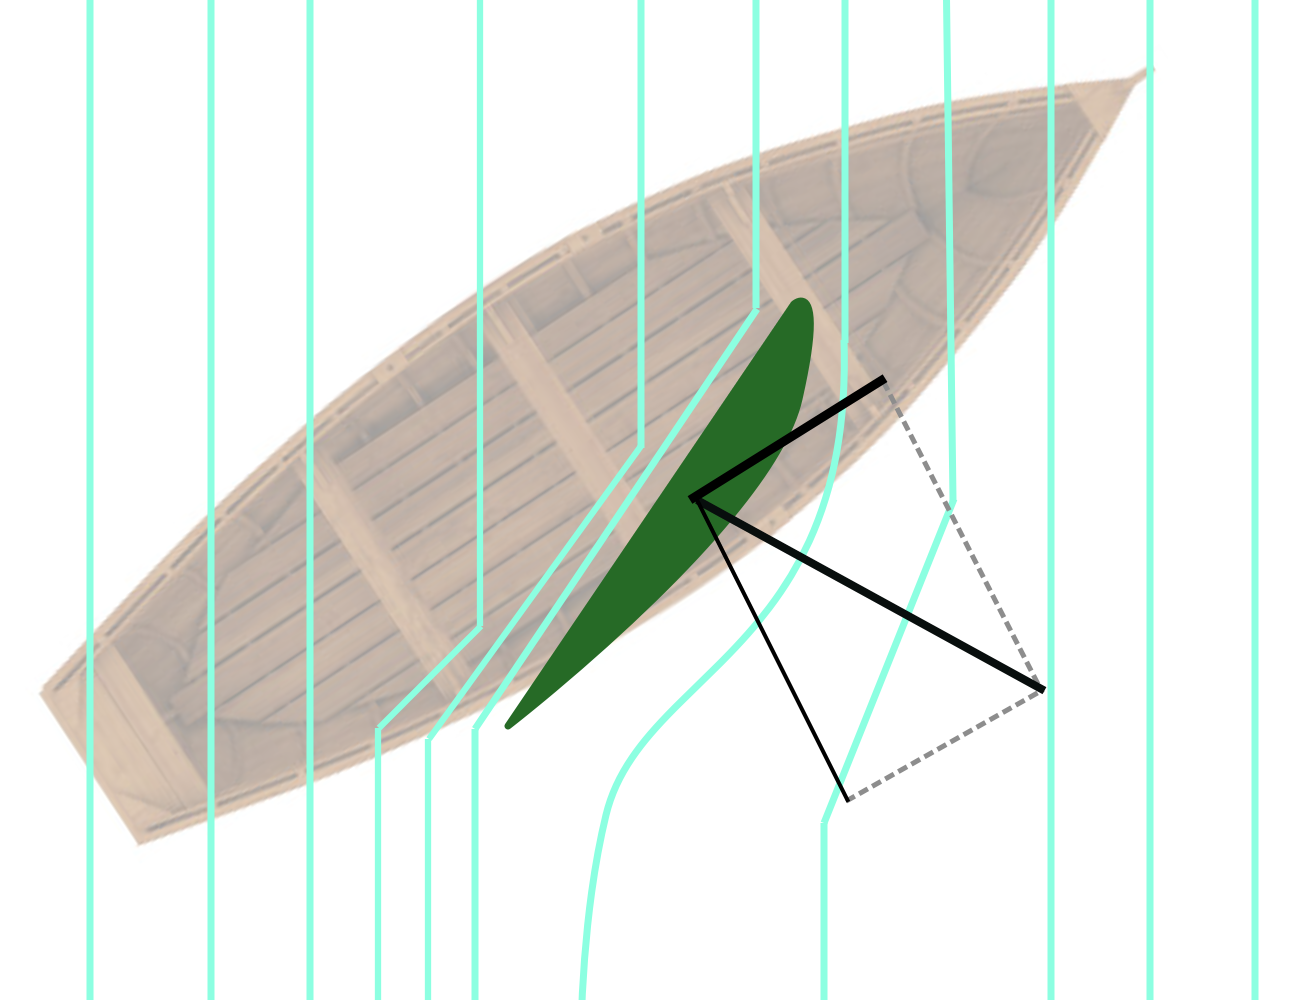
\includegraphics[width=.75\textwidth]{wing.png}
\end{center}

Of course, for the sail to work on either side of the boat,  this asymmetrical design would not work.  (Although,  we should note that this design works great
for airplane wings.)

When we make a sail out of cloth,  we give it some curve known as \newterm{camber}\index{camber}.  Slow winds require just a little camber;  fast winds require more.

\begin{center}
    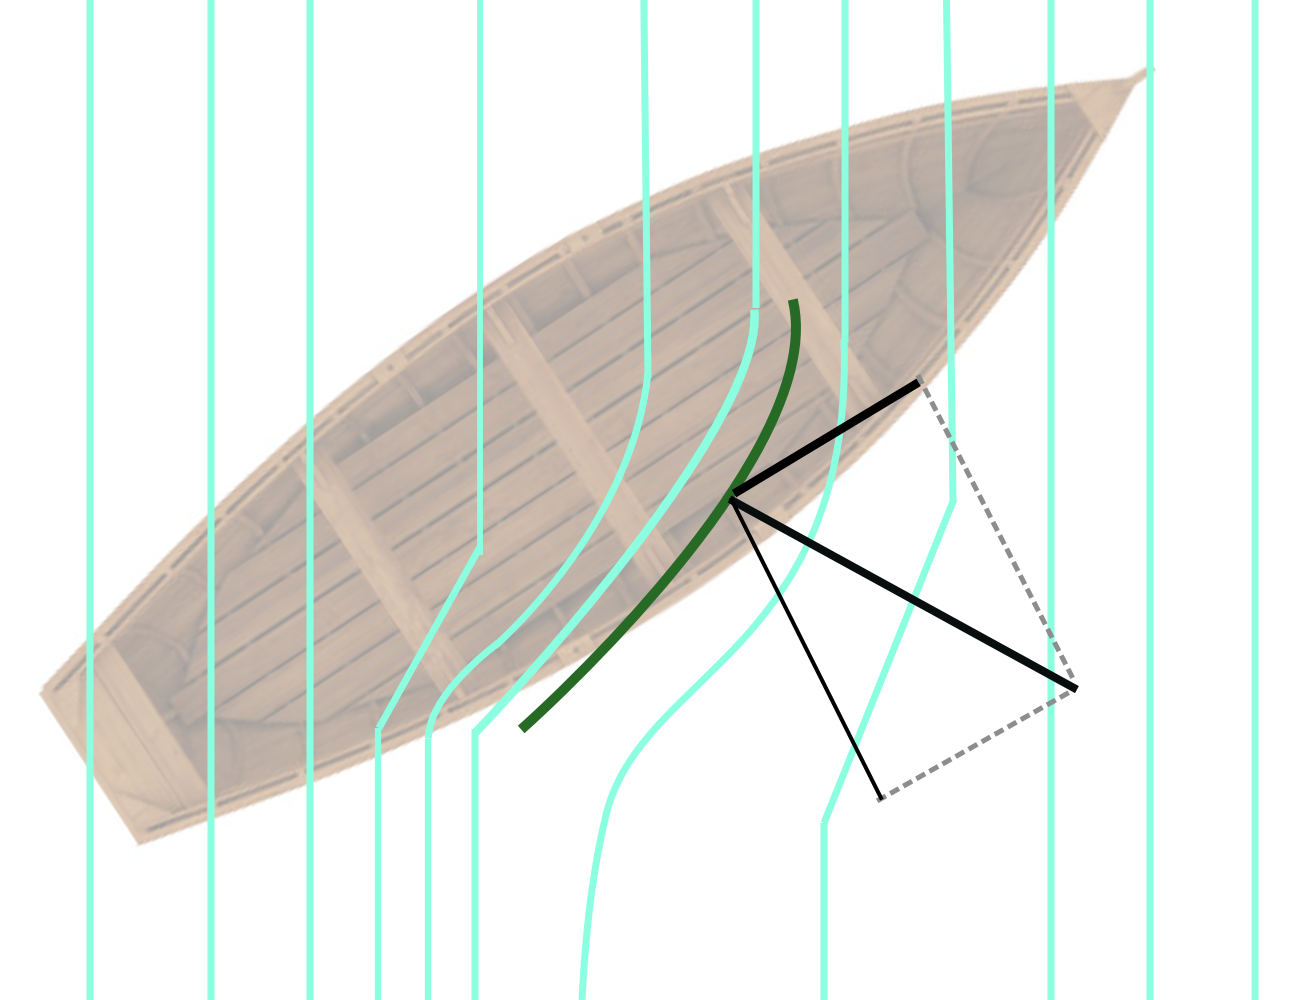
\includegraphics[width=.75\textwidth]{soft.png}
\end{center}


Some newer sailboats have wing sails that have two pieces that can be arranged to redirect the most air possible.

Note: when running with the wind,  the turbulence on the leeward side of the sail is unavoidable.   But when traveling perpendicular to the wind or on a close reach,  the air should move smoothly over the leeward side of the sail.   Many sailors have a piece of yarn taped on each side of the sail so they can see if the air is moving smoothly.

Many sailboats also have multiple sails.  Besides the increase in the sail area,  each sail also redirects the wind to pass smoothly over the leeward surface of the sail
behind it.
\index{tacking}
\subsection{Tacking into the Wind}

What if the wind is coming from the east and you really need to go directly into the wind?

The boat will not travel straight into the wind,  instead you will travel on a close reach with the wind coming from one side of the boat. You will then turn into the wind and continue turning
until you are on a close reach with the wind coming from the other side.  This is known as \newterm{tacking}.

\begin{center}
    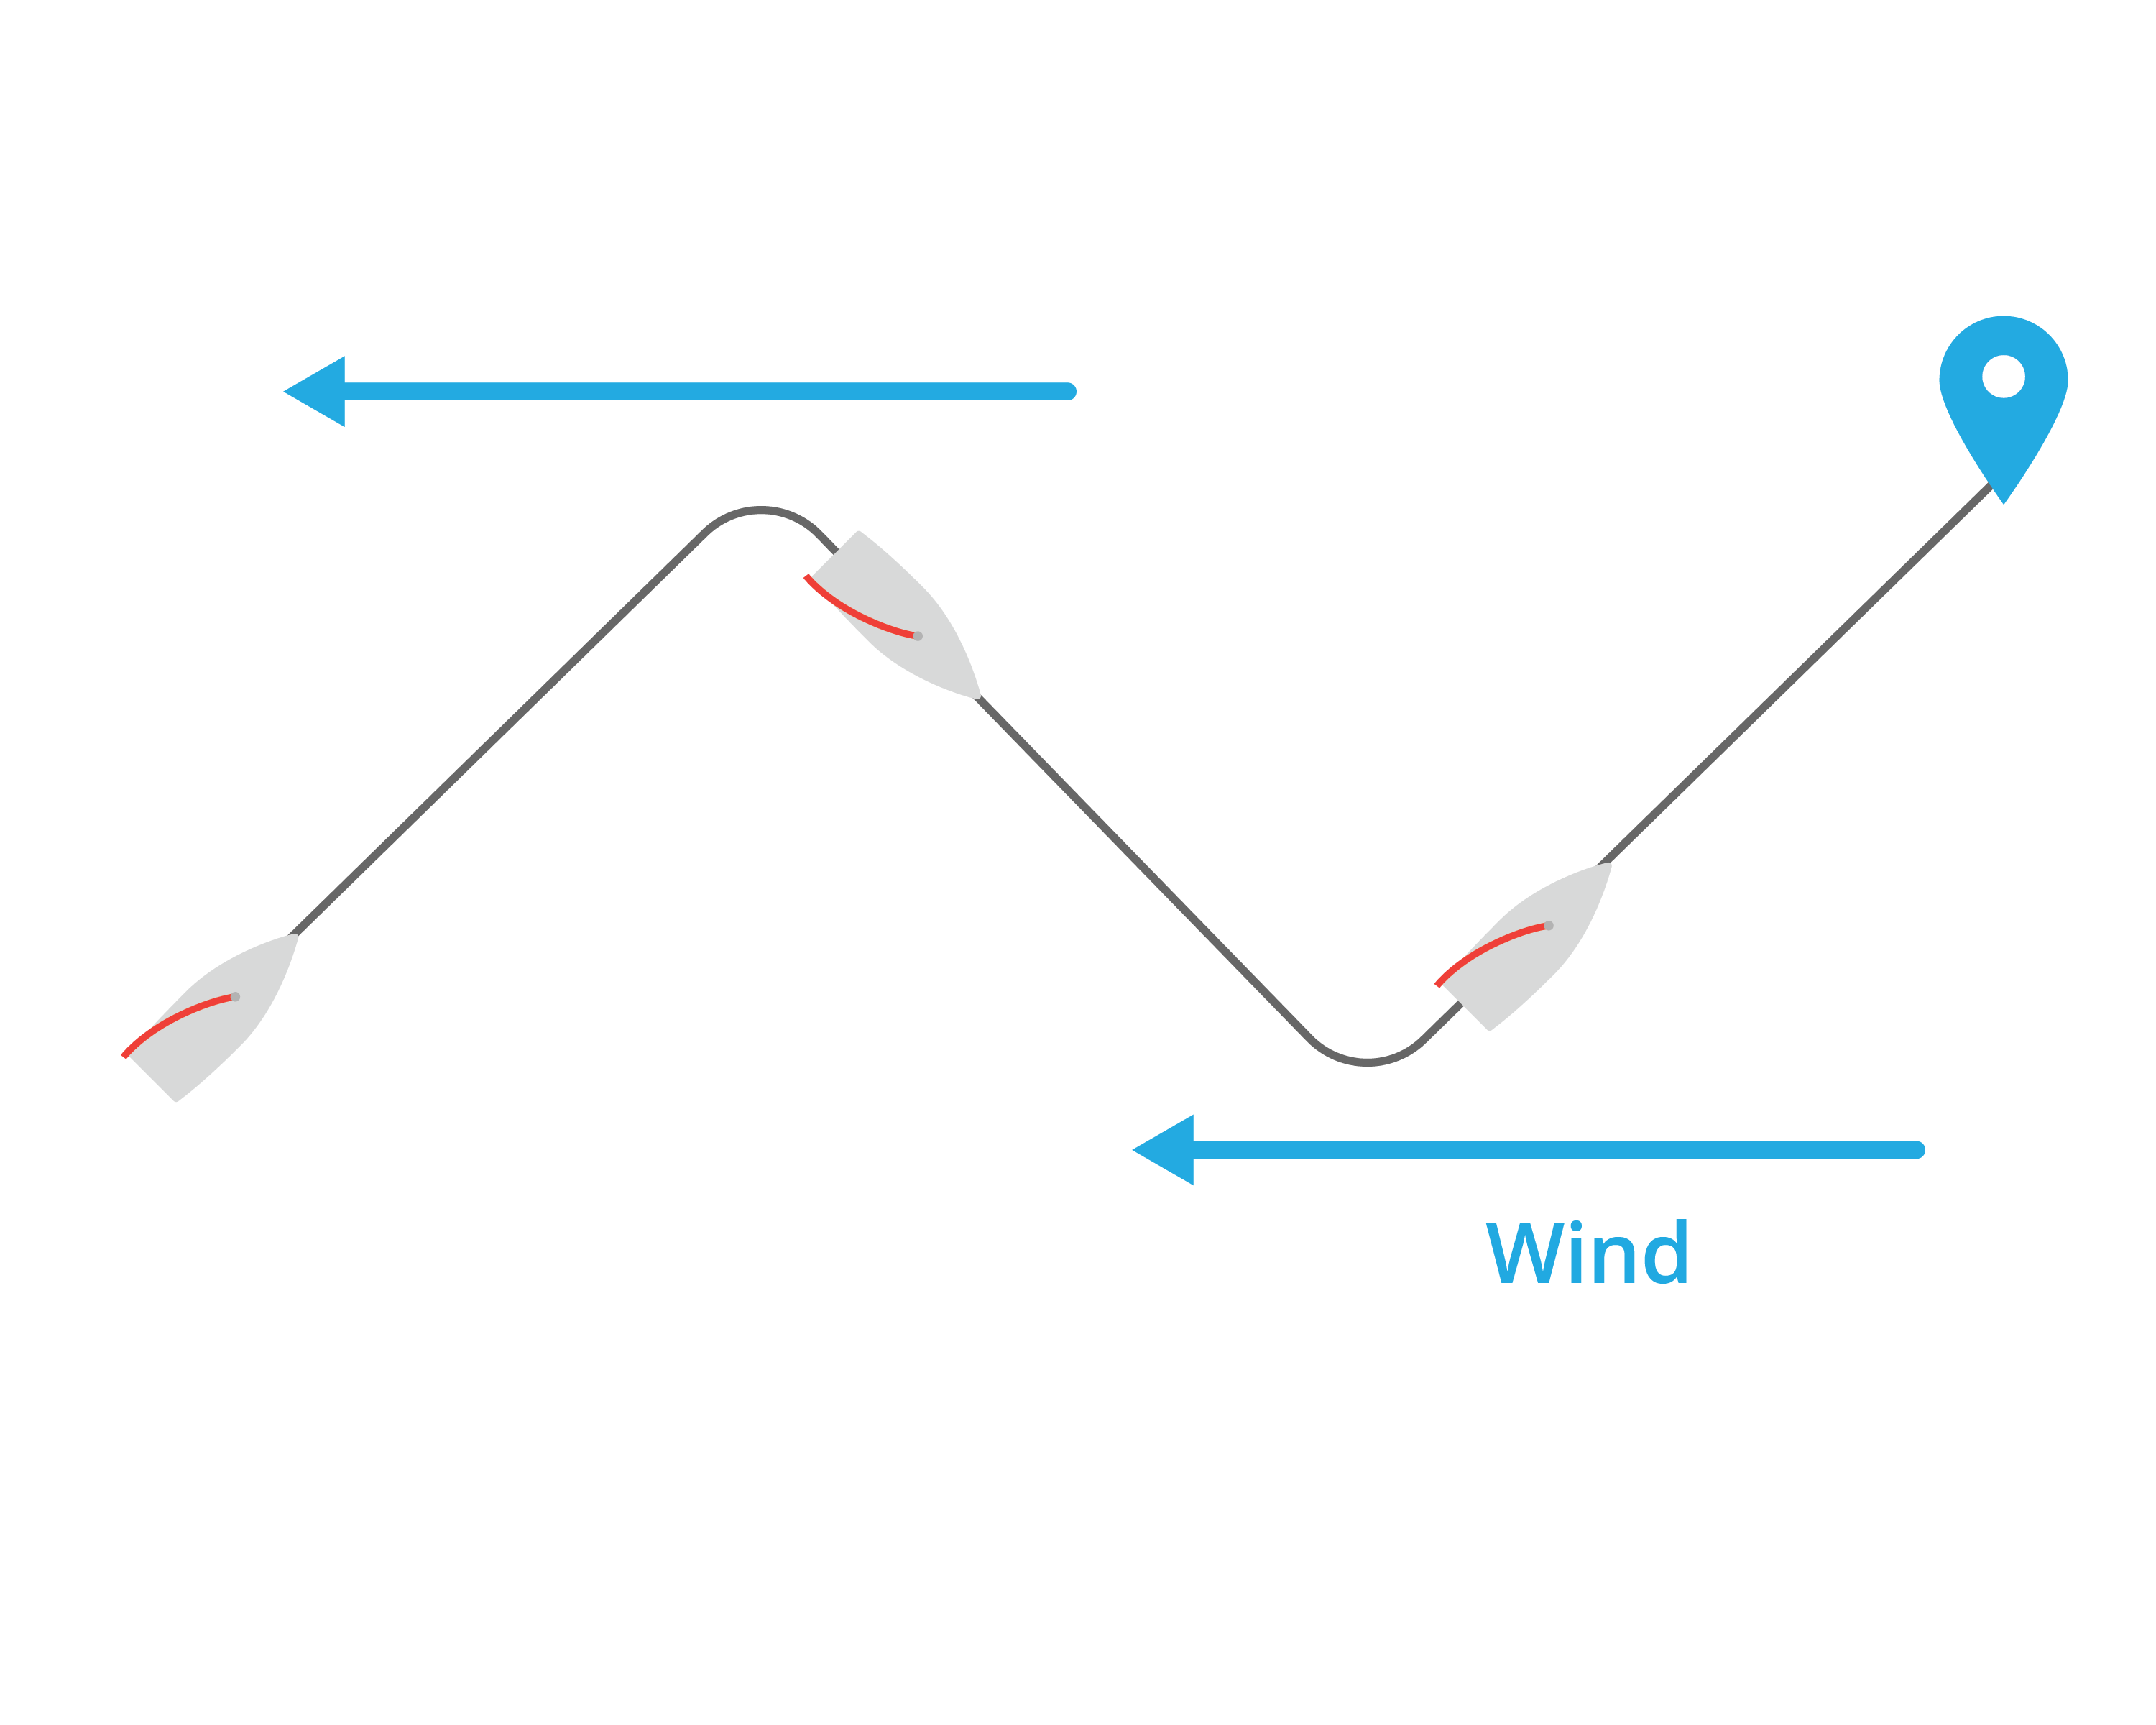
\includegraphics[width=.75\textwidth]{tacking.png}

\end{center}

\subsection{Heeling}

The center of effort is near the center of your sail,  which is usually pretty high in the air. Yes, the force generated will push your boat,  but it will also rotate your boat.  Sailors call
the resulting lean \newterm{heeling}\index{heeling}. Heeling too far is problematic --- the rudder gets pulled out of the water, which makes it hard to steer the boat.



If a boat is heeling too far,  sailors will move their weight to the windward side of the boat --- some even wear harnesses that push their weight out beyond the edge of the hull.
If that doesn't work, they will reduce the sideways force on the sail.

\begin{center}
    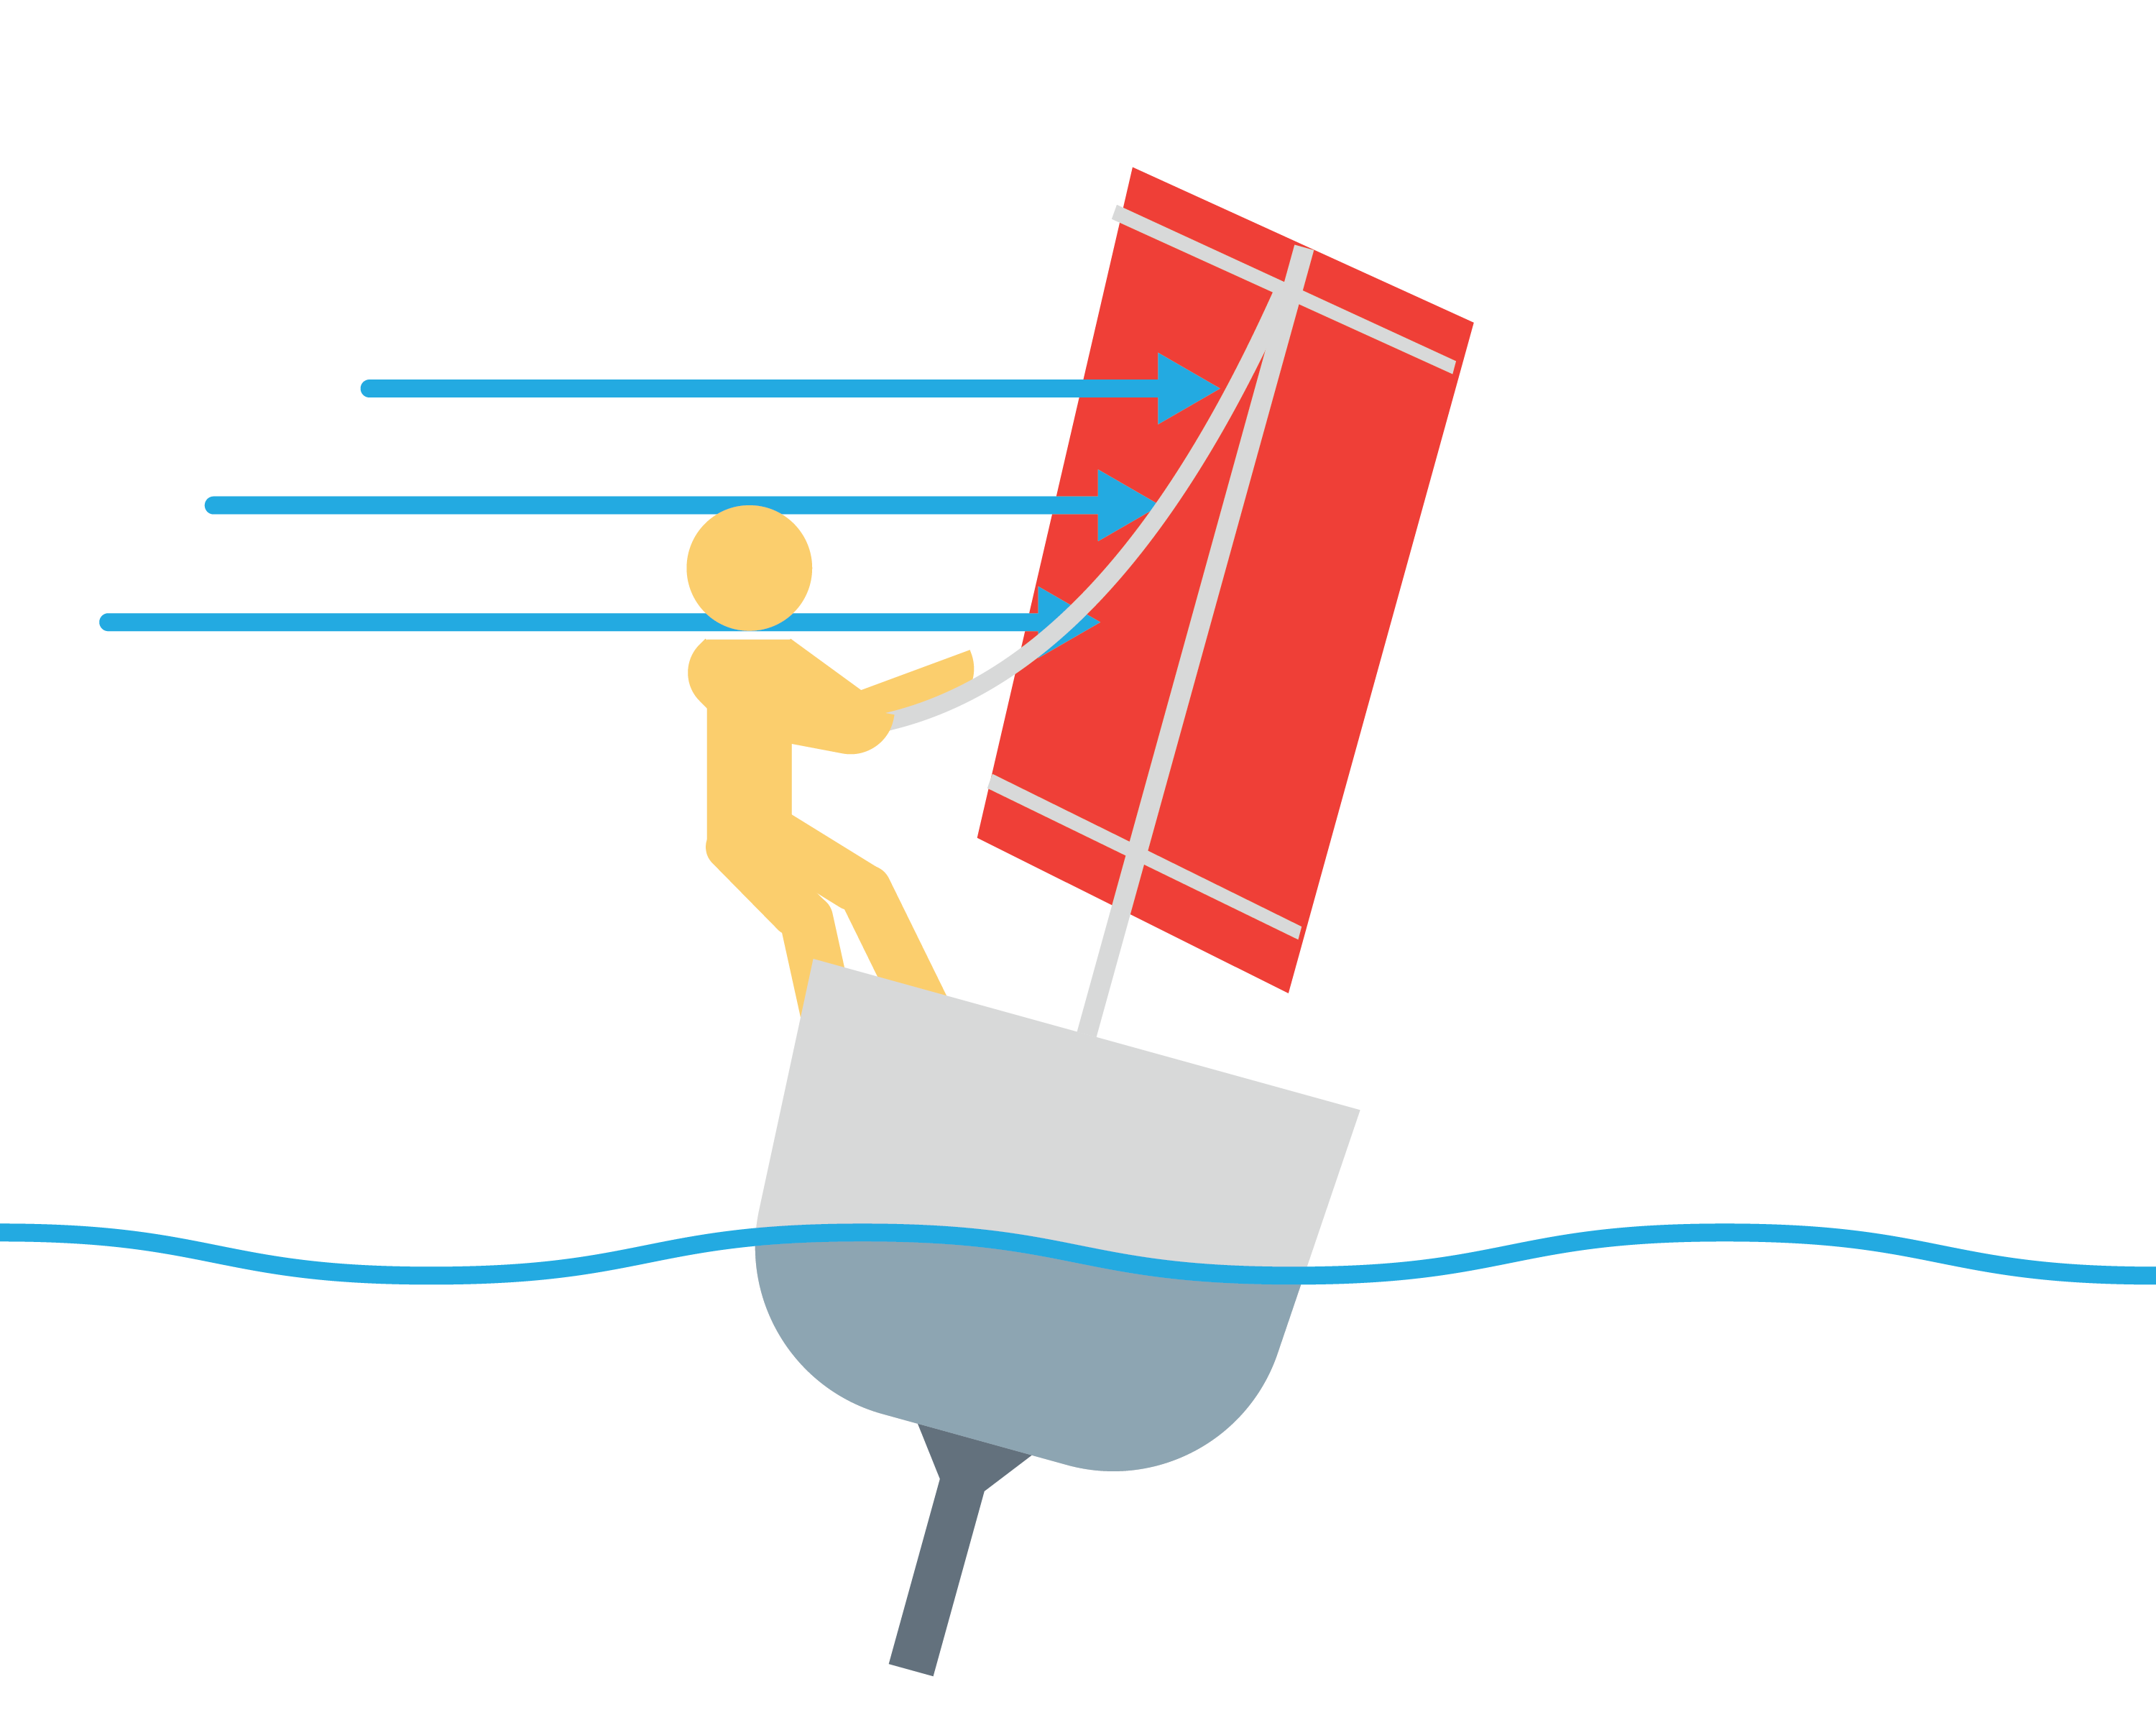
\includegraphics[width=.75\textwidth]{heeling2.png}

\end{center}

Can the boat flip over?  (The word sailors use is \newterm{capsize}\index{capsize}.)  Most larger boats should not be able to capsize; as the sail gets pushed down toward the water, it loses power.  So, putting some weight in the keel will ensure that the boat doesn't turn upside-down.  Small boats (think 3 or 4 meters long) can capsize,  but they are small enough that the sailor can usually
get them upright again without assistance.

There are boats with multiple hulls. A catamaran has two identical hulls that are side-by-side.  As a result,  the catamaran will not heel much at all.  However,  if a big gust of wind comes up, one hull can be pulled completely out of the water.  Catamarans can be capsized.

If a boat is running when a big gust comes up,  that rotating force will try to push the bow underwater. If the boat is going very fast,  this can result in a somersault as
the front of the boat slows and dips suddenly and the back of the boat is pitched up over it.

\begin{center}
    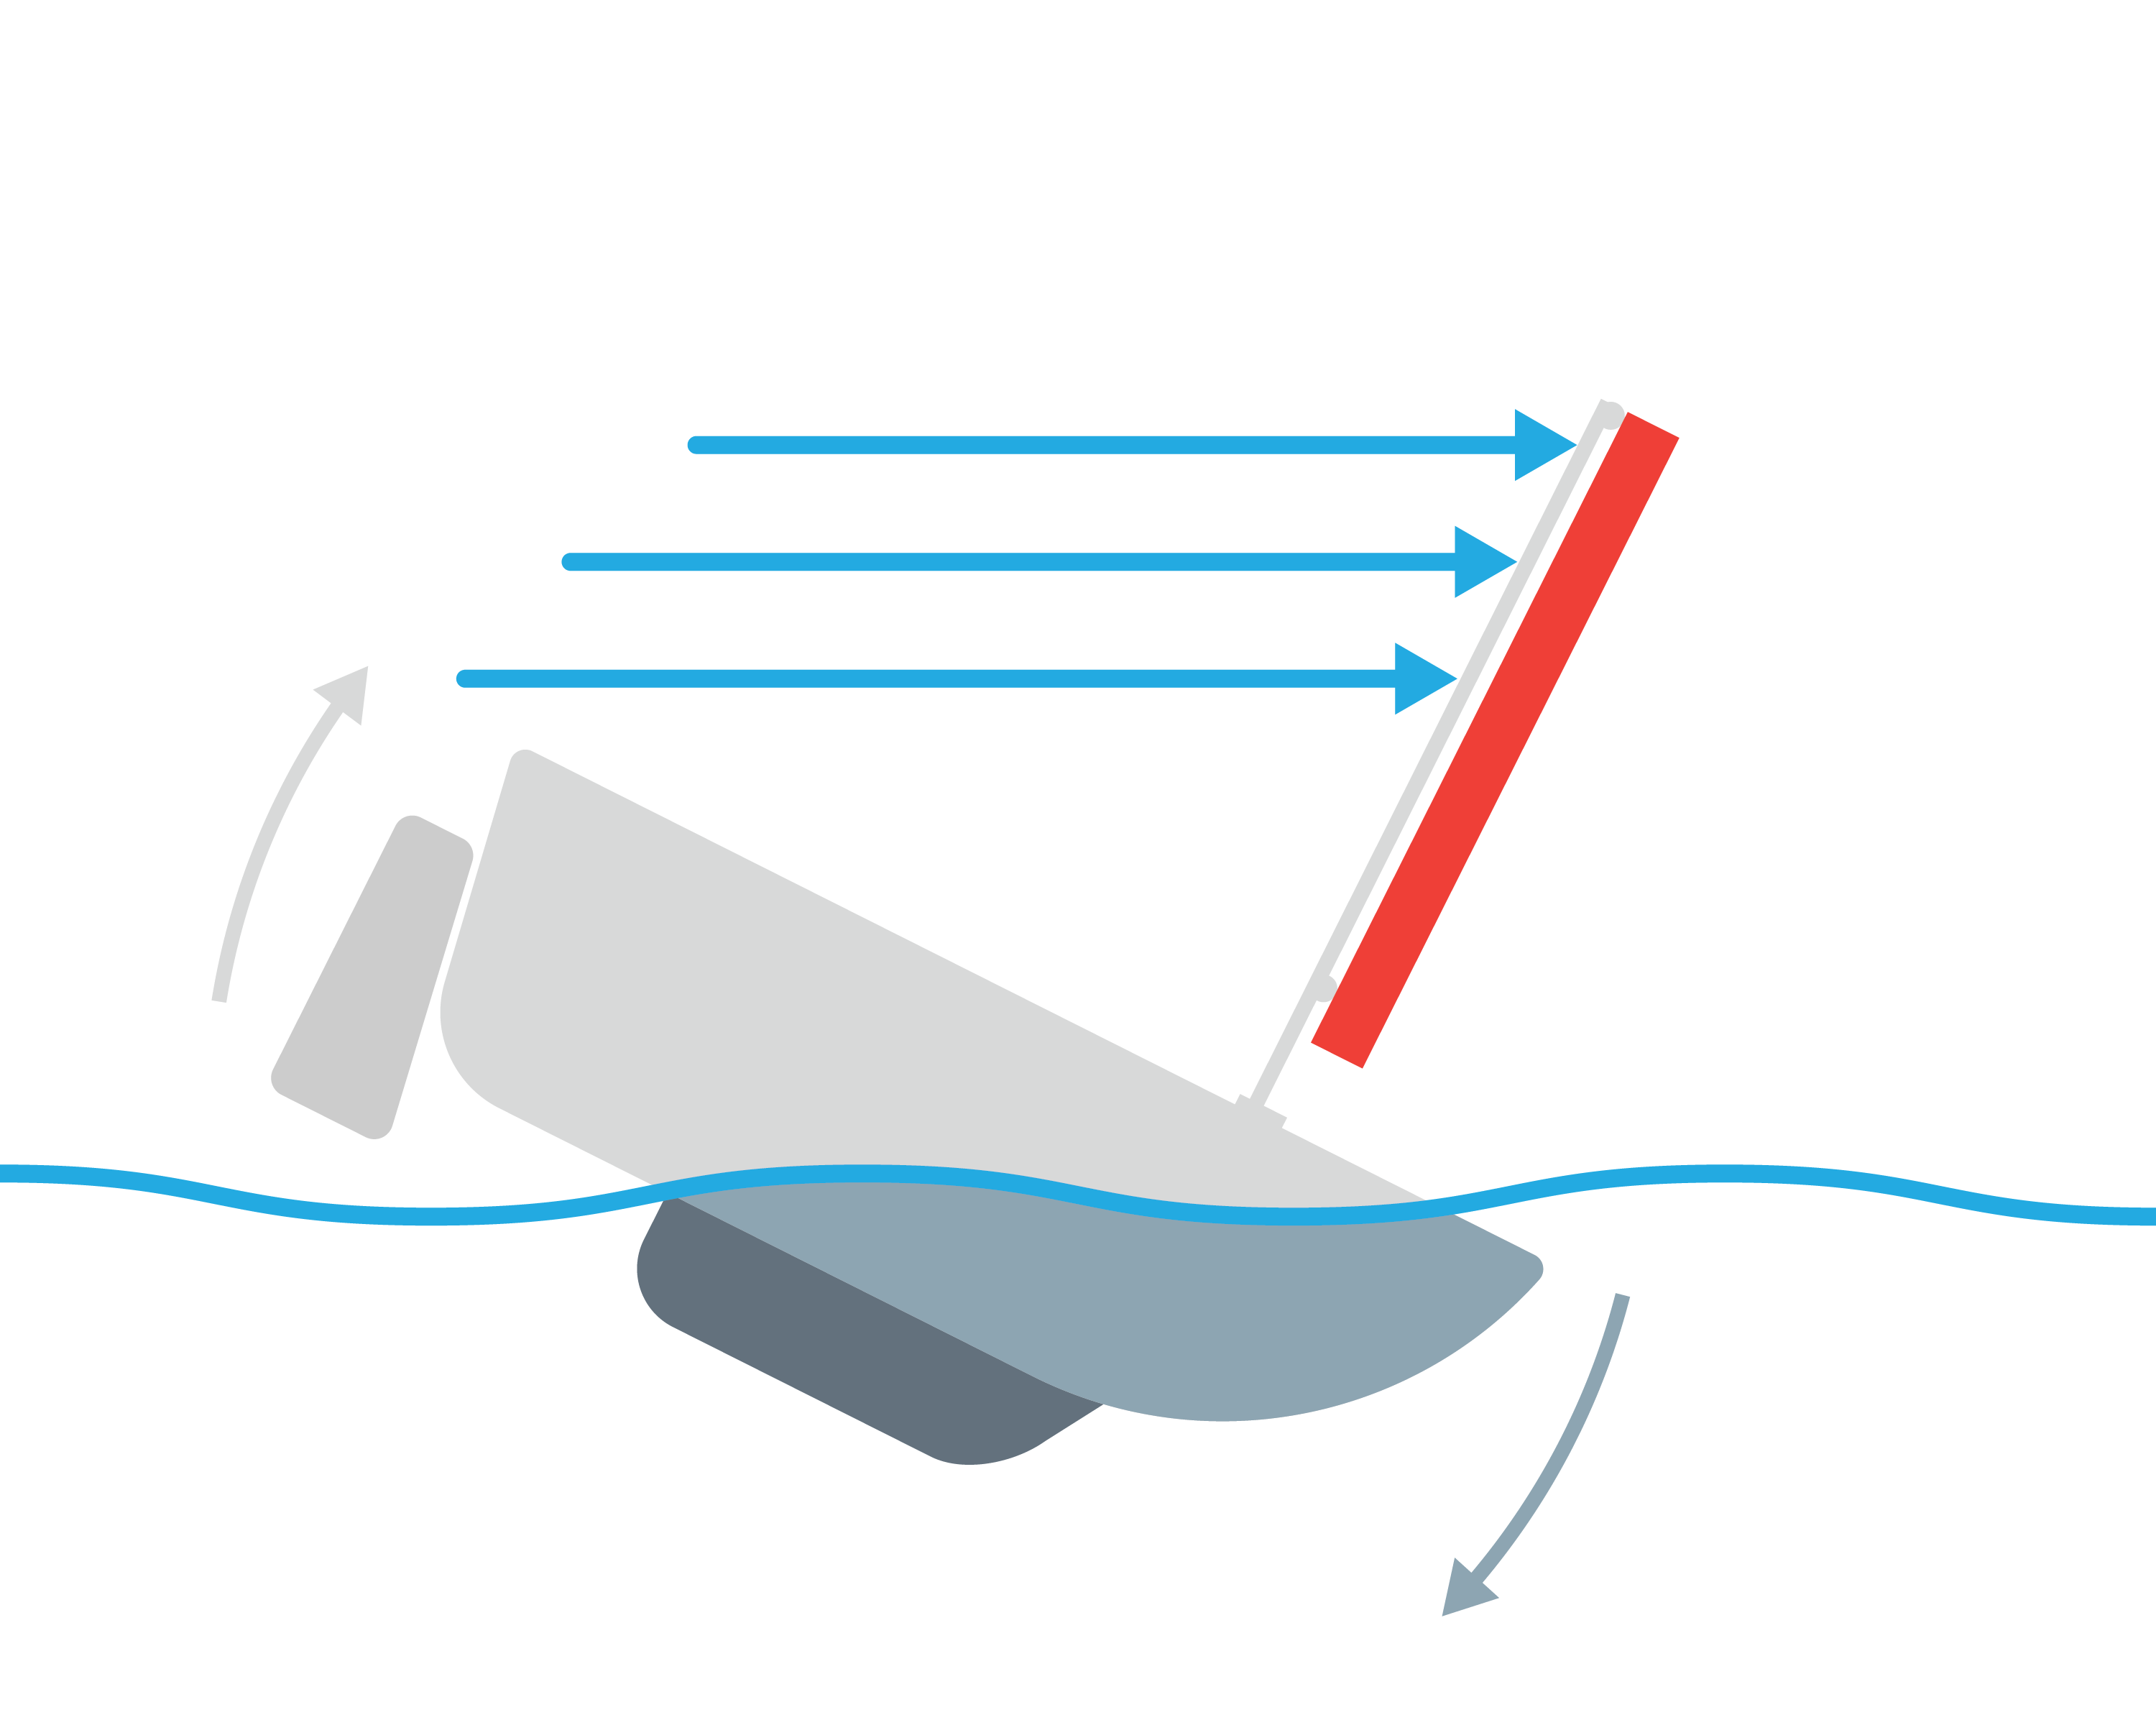
\includegraphics[width=.75\textwidth]{heeling.png}

\end{center}
